% Template KLTN cho SV trường ĐHKHTN
% Liên hệ: nqminh@fit.hcmus.edu.vn
% Last update: 08/06/2016

% Chú ý: đọc các phần chú ý đóng khung của file này và chỉnh lại cho phù hợp.
% Trước khi build, xóa hết các file được tạo ra trong quá trình build trước đó, và build theo thứ tự: BIB > PDF > PDF.
% Nếu cập nhật tài liệu tham khảo, cũng cần build lại theo cách trên.

\documentclass[twoside,a4paper,14pt]{extreport}
% font size
\usepackage[fontsize=13pt]{scrextend}
% Font tiếng Việt
\usepackage[T5]{fontenc}
\usepackage[utf8]{inputenc}
\DeclareTextSymbolDefault{\DH}{T1}

% Tài liệu tham khảo
\usepackage[
	sorting=none,
	backend=bibtex,
	defernumbers=true]{biblatex}
\usepackage[unicode]{hyperref} % Bookmark tiếng Việt
\addbibresource{References/references.bib}

\makeatletter
\def\blx@maxline{77}
\makeatother

% Chèn hình, các hình trong luận văn được để trong thư mục Images/
\usepackage{graphicx}
\graphicspath{ {Images/} }
\usepackage{caption}
\usepackage[export]{adjustbox}

% Chèn và định dạng mã nguồn
\usepackage{listings}
\usepackage{color}
\definecolor{codegreen}{rgb}{0,0.6,0}
\definecolor{codegray}{rgb}{0.5,0.5,0.5}
\definecolor{codepurple}{rgb}{0.58,0,0.82}
\definecolor{backcolour}{rgb}{0.95,0.95,0.92}
\lstdefinestyle{mystyle}{
    backgroundcolor=\color{backcolour},   
    commentstyle=\color{codegreen},
    keywordstyle=\color{magenta},
    numberstyle=\tiny\color{codegray},
    stringstyle=\color{codepurple},
    basicstyle=\footnotesize,
    breakatwhitespace=false,         
    breaklines=true,                 
    captionpos=b,                    
    keepspaces=true,                 
    numbers=left,                    
    numbersep=5pt,                  
    showspaces=false,                
    showstringspaces=false,
    showtabs=false,                  
    tabsize=2
}
\lstset{style=mystyle}

% Chèn và định dạng mã giả
\usepackage{amsmath}
\usepackage{algorithm}
\usepackage[noend]{algpseudocode}
\makeatletter
\def\BState{\State\hskip-\ALG@thistlm}
\makeatother

% Bảng biểu
\usepackage{multirow}
\usepackage{array}
\newcolumntype{L}[1]{>{\raggedright\let\newline\\\arraybackslash\hspace{0pt}}m{#1}}
\newcolumntype{C}[1]{>{\centering\let\newline\\\arraybackslash\hspace{0pt}}m{#1}}
\newcolumntype{R}[1]{>{\raggedleft\let\newline\\\arraybackslash\hspace{0pt}}m{#1}}
 
% Đổi tên mặc định
\renewcommand{\chaptername}{CHƯƠNG}
\renewcommand{\figurename}{Hình}
\renewcommand{\tablename}{Bảng}
\renewcommand{\contentsname}{MỤC LỤC}
\renewcommand{\listfigurename}{DANH SÁCH CÁC HÌNH}
\renewcommand{\listtablename}{DANH SÁCH CÁC BẢNG}
\renewcommand{\appendixname}{PHỤ LỤC}

% Định dạng chapter
\usepackage{titlesec}

\setcounter{secnumdepth}{3}

\titleformat{\chapter}
    [block]
    {\filcenter\normalfont\bfseries\normalsize}{\chaptername \ \thechapter :}{10pt}{\normalsize}
\titlespacing*{\chapter}{0pt}{-10pt}{10pt} %khoảng cách giữa chapter và đầu trang

\titleformat{\section}
    {\normalfont\bfseries\normalsize}{\thesection}{1em}{}
 
\titleformat{\subsection}
    {\normalfont\bfseries\normalsize}{\thesubsection}{1em}{}

\titleformat{\subsubsection}
    {\normalfont\bfseries\normalsize}{\thesubsubsection}{1em}{}

% Dãn dòng 1.5
\usepackage{setspace}
\onehalfspacing

% Thụt vào đầu dòng
\usepackage{indentfirst}

% Bottom right page numbering
\usepackage{fancyhdr} % for use of \pageref{LastPage}
\pagestyle{fancy} % Turn on the style
\fancyhf{} % Start with clearing everything in the header and footer
% Set the right side of the footer to be the page number
\fancyfoot[R]{\thepage}
\renewcommand{\headrulewidth}{0pt}%
% Redefine plain style, which is used for titlepage and chapter beginnings
% From https://tex.stackexchange.com/a/30230/828
\fancypagestyle{plain}{%
    \renewcommand{\headrulewidth}{0pt}%
    \fancyhf{}%
    \fancyfoot[R]{\thepage}%
}

% Canh lề
\usepackage[
  twoside,
  top=20mm,
  bottom=20mm,
  left=25mm,
  right=20mm,
  footskip = 15mm,
  includefoot]{geometry}

% Trang bìa
\usepackage{tikz}
\usetikzlibrary{calc}
\newcommand\HRule{\rule{\textwidth}{1pt}}

% Danh sách chữ viết tắt
\usepackage{myacronyms}

\newcommand\myemptypage{
\newpage
\thispagestyle{empty}
\mbox{}
\newpage
}

% ========================================================================================= %
% CHÚ Ý: Thông tin chung về KLTN - sinh viên điền vào đây để tự động update các trang khác  %
% ========================================================================================= %
\newcommand{\tenSV}{Nguyễn~Vũ~Minh~Thành} % Dấu ~ là khoảng trắng không được tách (các chữ nối với nhau bằng dấu ~ sẽ nằm cùng 1 dòng
\newcommand{\mssv}{19207103}
\newcommand{\tenKL}{THỰC HIỆN NỀN TẢNG IOT SỬ DỤNG HỆ~THỐNG~BACK-END GIAO~TIẾP PHẦN~CỨNG QUA~WIFI KẾT~HỢP KỸ~THUẬT MẬT~MÃ~HÓA~NHẸ} % Chú ý dấu ~ trong tên khóa luận
\newcommand{\tenGVHD}{TS.~Lê~Đức~Hùng}
\newcommand{\tenBM}{}

\begin{document}

% fix anchor bug
\hypersetup{pageanchor=false}
\begin{titlepage}

\begin{center}
ĐẠI HỌC QUỐC GIA THÀNH PHỐ HỒ CHÍ MINH\\
TRƯỜNG ĐẠI HỌC KHOA HỌC TỰ NHIÊN\\
\textbf{KHOA ĐIỆN TỬ - VIỄN THÔNG}\\[2cm]


{ \Large \bfseries Nguyễn Vũ Minh Thành\\[2cm] } 

%Tên đề tài Khóa luận tốt nghiệp/Đồ án tốt nghiệp

{ \Large \bfseries THỰC HIỆN NỀN TẢNG IOT CLOUD GIAO~TIẾP PHẦN CỨNG KẾT HỢP KỸ~THUẬT MẬT MÃ HÓA NHẸ \\[3cm]} 


%Chọn trong các dòng sau
\large KHÓA LUẬN TỐT NGHIỆP CỬ NHÂN\\
%\large ĐỒ ÁN TỐT NGHIỆP CỬ NHÂN\\
%\large THỰC TẬP TỐT NGHIỆP CỬ NHÂN\\
\large NGÀNH KỸ THUẬT ĐIỆN TỬ-VIỄN THÔNG\\
%Đưa vào dòng này nếu thuộc chương trình Chất lượng cao, hoặc lớp Cử nhân tài năng
% \large CHƯƠNG TRÌNH CHÍNH QUY\\
\large CHƯƠNG TRÌNH CHẤT LƯỢNG CAO\\
%\large CHƯƠNG TRÌNH CỬ NHÂN TÀI NĂNG\\[2cm]


\begin{tikzpicture}[remember picture, overlay]
  \draw[line width = 2pt] ($(current page.north west) + (2cm,-2cm)$) rectangle ($(current page.south east) + (-1.5cm,2cm)$);
\end{tikzpicture}

\vfill
Tp. Hồ Chí Minh, tháng 07/2023

\end{center}

\pagebreak



\begin{center}
ĐẠI HỌC QUỐC GIA THÀNH PHỐ HỒ CHÍ MINH\\
TRƯỜNG ĐẠI HỌC KHOA HỌC TỰ NHIÊN\\
\textbf{KHOA ĐIỆN TỬ - VIỄN THÔNG}\\[2cm]


{\large \bfseries Nguyễn Vũ Minh Thành - 19207103\\[2cm]}

%Tên đề tài Khóa luận tốt nghiệp/Đồ án tốt nghiệp

{ \Large \bfseries THỰC HIỆN NỀN TẢNG IOT CLOUD GIAO~TIẾP PHẦN CỨNG KẾT HỢP KỸ~THUẬT MẬT MÃ HÓA NHẸ\\[2cm] } 


%Chọn trong các dòng sau
\large KHÓA LUẬN TỐT NGHIỆP CỬ NHÂN\\
%\large ĐỒ ÁN TỐT NGHIỆP CỬ NHÂN\\
\large NGÀNH KỸ THUẬT ĐIỆN TỬ-VIỄN THÔNG\\
%Đưa vào dòng này nếu thuộc chương trình Chất lượng cao, hoặc lớp Cử nhân tài năng
% \large CHƯƠNG TRÌNH CHÍNH QUY\\[2cm]
\large CHƯƠNG TRÌNH CHẤT LƯỢNG CAO\\[2cm]
%\large CHƯƠNG TRÌNH CỬ NHÂN TÀI NĂNG\\[2cm]

\textbf{NGƯỜI HƯỚNG DẪN KHOA HỌC}\\
TS. Lê Đức Hùng

\begin{tikzpicture}[remember picture, overlay]
  \draw[line width = 2pt] ($(current page.north west) + (2cm,-2cm)$) rectangle ($(current page.south east) + (-1.5cm,2cm)$);
\end{tikzpicture}

\vfill
Tp. Hồ Chí Minh, tháng 07/2023

\end{center}
\thispagestyle{empty}
\end{titlepage}
\hypersetup{pageanchor=true}
% Sasu trang Title, các bạn chèn nhận xét gủa GVHD và GVPB. Nhận xét sẽ được giáo vụ phát sau buổi bảo vệ để các bạn đóng quyển.

\pagenumbering{roman} % Đánh số i, ii, iii, ...

%\addcontentsline{toc}{chapter}{Lời cam đoan}
%\chapter*{Lời cam đoan}
\label{reassurances}

Tôi xin cam đoan đây là công trình nghiên cứu của riêng tôi. Các số liệu và kết quả nghiên cứu trong luận văn này là trung thực và không trùng lặp với các đề tài khác.

\newpage
\phantomsection
\addcontentsline{toc}{chapter}{LỜI CẢM ƠN}
\begin{frame}
    \begin{center}
        {\Huge\calligra Thank you for your attention!}
    \end{center}
\end{frame}

\newpage
\phantomsection
\addcontentsline{toc}{chapter}{ABSTRACT}
\chapter*{ABSTRACT}
\label{Abstract-EN}
\addcontentsline{toc}{chapter}{ABSTRACT}

% Context, Problems
To assist managers of the \acrfull{vnpt} Tien Giang in monitoring \glspl{bts}, an \acrfull{iot} system and model were required to be constructed. The system must develop communication and synchronization techniques between sensors, physical devices, and a database in a \acrfull{vps}, as well as a customized graphical user interface for data visualization.
% Objectives
To achieve the above objectives, the \acrshort{iot} system will be constructed using a \acrfull{mcu} communicating things; server applications managing data; a customizable graphical interface; communication and synchronization mechanisms; and lightweight cryptography.
% Phương pháp
The \acrshort{iot} system uses STM32 \acrshort{mcu} communicating things, ESP32 \acrshort{iot} gateway, self-designed protocol, and lightweight cryptography ChaCha20-Poly1305. The system runs server applications on the \acrshort{vps}, including an \acrshort{api} server, a \acrfull{mqtt} broker, and a MongoDB database, as well as a web server with a graphical interface.
% Kết quả
In the sensing system, STM32 \acrshort{mcu} has communication and synchronization mechanisms with the back-end system, and the ESP32 gateway has a data-routing mechanism. Server applications are built in the \acrshort{vps} via Docker Containerization, an Nginx web server administers and provides a web interface, and cryptography is applied during the gateway-\acrshort{api} server transfer.
% Kết luận
The suggested \acrshort{iot} system has a model that is suited for communication and synchronization methods between devices, gateways, and the back-end system; the web interface is versatile in terms of creating and displaying widgets. The lightweight cryptographic algorithm assures data security between the gateway and the back-end system, and the protocol includes a dependable structure for frame detection and error detection.


\newpage
\phantomsection
\addcontentsline{toc}{chapter}{TÓM TẮT}
\chapter*{TÓM TẮT}
\label{Abstract}

% Ngữ cảnh, vấn đề
Một hệ thống và mô hình \acrfull{iot} được yêu cầu xây dựng để giúp các quản trị viên \acrfull{vnpt} Tiền Giang giám sát các \acrfull{bts}. Hệ thống phải tạo ra cơ chế giao tiếp và đồng bộ giữa các cảm biến và thiết bị vật lý với cơ sở dữ liệu trên máy chủ ảo và giao diện người dùng linh hoạt để trực quan hóa dữ liệu. 
% Mục tiêu
Hệ thống \acrshort{iot} sử dụng \acrfull{vdk} giao tiếp vạn vật, các ứng dụng server xử lý dữ liệu, giao diện linh hoạt và mật mã hóa nhẹ, sẽ được xây dựng để phục vụ cho các yêu cầu trên. 
% Phương pháp
Hệ thống sử dụng \acrshort{vdk} STM32 giao tiếp vạn vật, \acrshort{iot} gateway ESP32, giao thức tự thiết kế, và mật mã hóa nhẹ ChaCha20-Poly1305. Trên máy chủ ảo, hệ thống vận hành các ứng dụng server: \acrfull{api} server, MQTT Broker và cơ sở dữ liệu MongoDB; và máy chủ web cung cấp giao diện người dùng. 
% Kết quả
Trên hệ thống vạn vật, \acrshort{vdk} STM32 đã có cơ chế giao tiếp và đồng bộ dữ liệu với cloud, gateway ESP32 có cơ chế chuyển tiếp dữ liệu. Trên máy chủ ảo, các ứng dụng server được triển khai bằng kỹ thuật Docker Containerizing, máy chủ web Nginx quản lý và cung cấp giao diện web, và mã hóa nhẹ được sử dụng giữa gateway và \acrshort{api} server. 
% Kết luận
Hệ thống \acrshort{iot} đưa ra có mô hình phù hợp với cơ chế giao tiếp và đồng bộ giữa thiết bị, gateway, và cloud, giao diện web có sự linh hoạt trong việc tạo và hiển thị các widget. Về việc giao tiếp, thuật toán mã hóa nhẹ đảm bảo việc bảo mật dữ liệu giữa gateway và cloud và giao thức có cấu trúc linh hoạt trong việc nhận diện và phát hiện lỗi.

% \phantomsection
% \addcontentsline{toc}{chapter}{Đề cương chi tiết}
% \include{Appendix/decuong}

% Mục lục, danh sách hình, danh sách bảng
\phantomsection
\addcontentsline{toc}{chapter}{MỤC LỤC}
\tableofcontents
% Danh sách chữ viết tắt
\printglossary[type=\acronymtype,
                title=DANH SÁCH CHỮ VIẾT TẮT, 
                toctitle=DANH SÁCH CHỮ VIẾT TẮT
                ]
\newpage
\phantomsection
\addcontentsline{toc}{chapter}{\listfigurename}
\listoffigures

\newpage
\phantomsection
\addcontentsline{toc}{chapter}{\listtablename}
\listoftables

\cleardoublepage

\pagenumbering{arabic} % Đánh số 1, 2, 3, ...

% Các chương nội dung
\chapter{GIỚI THIỆU}
\label{Chapter1}

\section{Đặt vấn đề}

% Ngữ cảnh, vấn đề cần giải quyết là gì?
Các quản trị viên \acrfull{vnpt} yêu cầu xây dựng hệ thống \acrfull{iot} giám sát các \acrfull{bts}. Hệ thống \acrshort{iot} phải cung cấp bo mạch giám sát thông số của các trạm \acrshort{bts}, giao diện người dùng dựa trên cơ sở dữ liệu của \acrfull{vps}, và có sử dụng mật mã hóa.

Trong quá trình phát triển, mô hình hệ thống phần cứng và các cơ chế giao tiếp và đồng bộ trên phần cứng phải được thiết kế. Tại \acrshort{vps}, mô hình hệ thống back-end và nền tảng giao diện người dùng phải được xác định. Bên cạnh đó, hệ thống phải đưa ra loại mật mã hóa được sử dụng. Trong quá trình hoạt động, bo mạch in phải được thiết kế để phù hợp với việc giám thông số của trạm \acrshort{bts} và có thể triển khai cơ chế đồng bộ với \acrshort{iot} cloud. Tại \acrshort{vps}, kỹ thuật triển khai hệ thống back-end và nền tảng giao diện phải được đưa ra. Cuối cùng, hệ thống \acrshort{iot} phải đưa ra cách thức triển khai kỹ thuật mật mã hóa.

% Vì sao vấn đề/bài toán quan trọng và thú vị?
    % Quản trị viên VNPT muốn giám sát BTS online.
Khi yêu cầu xây dựng hệ thống \acrshort{iot}, các quản trị viên muốn giám sát trạm \acrshort{bts} online thay vì giám sát trực tiếp. Chính vì vậy, hệ thống \acrshort{iot} sẽ phục vụ cho việc giảm thiểu việc giám sát trạm \acrshort{bts} offline và chi phí di chuyển tới trạm. 
    % Hệ thống IoT giải quyết vấn đề của BTS và các vấn đề khác.
Không chỉ phục vụ cho việc giám sát trạm \acrshort{bts}, hệ thống \acrshort{iot} sẽ được xây dựng với cấu trúc linh hoạt để phục vụ nhiều loại hệ thống giám sát và điều khiển online.

% Bài toán có gì khó? Vì sao cần phải giải quyết?
    % Cơ chế giao tiếp và đồng bộ đáng tin cậy và tự phục hồi
    % Giao diện người dùng phải linh hoạt để dễ dàng thay đổi các thành phần hiển thị.
    % Hệ thống back-end phải đồng bộ các dữ liệu của cơ sở dữ liệu với giao diện và bo mạch.
    % Giúp cài đặt cơ chế đồng bộ và giao tiếp trên toàn hệ thống. Triển khai mật mã nhẹ một cách hợp lý
Trong việc giao tiếp, hệ thống phải có cơ chế giao tiếp và đồng bộ đáng tin cậy và có khả năng tự phục hồi. Hơn nữa, giao diện người dùng phải linh hoạt để dễ dàng thay đổi các thành phần hiển thị của người dùng. Sau cùng, hệ thống back-end phải có cơ chế đồng bộ dữ liệu với giao diện và bo mạch một cách đáng tin cậy. Khi giải quyết được các vấn đề trên, cơ chế giao tiếp và đồng bộ có thể triển khai trên toàn hệ thống và có thể triển khai mật mã hóa hợp lý.

\section{Mục tiêu}

% Thiết kế bo mạch sử dụng vi điều khiển và phù hợp với việc giám sát BTS.
% Thiết kế cơ chế đồng bộ đáng tin cậy và có khả năng tự phục hồi. Cấu trúc frame có các thành phần nhận diện và phát hiển lỗi.
% Giao diện web linh hoạt có thể tùy chỉnh các thành phần hiển thị.
% Mật mã hóa được triển khai hợp lý trên cơ sở giao tiếp.
% Thiết kế hệ thống back-end có cơ sở dữ liệu, API server, và web-server.
Bo mạch được thiết kế sử dụng \acrfull{mcu} cấu tạo nên các thiết bị và gateway phù hợp với viêc giám sát \acrshort{bts}. Về việc giao tiếp, cơ chế đồng bộ được xây dựng đáng tin cậy và có khả năng tự phục hồi. Hơn nữa, cấu trúc frame giao tiếp được tạo nên có các thành phần nhận diện frame và phát hiện lỗi. Về bảo mật, mật mã hóa được triển khai hợp lý trên cơ sở giao tiếp của hệ thống. Về giao diện, hệ thống cung cấp giao diện web linh hoạt có thể tùy chỉnh các thành phần hiển thị. Về hệ thống back-end, back-end cung cấp cơ sở dữ liệu, \acrshort{api} server, broker server, và web-server.

\section{Giải pháp}

% Những giải pháp (nghiên cứu, ứng dụng) đã giải quyết bài toán này?
    % Các IoT Cloud như Blynk, ThingsBoard được sử dụng để thu nhận và trực quan hóa dữ liệu từ bo mạch.
    % Sử dụng vi điều khiển ESP Station ở chế độ Web-Server.
Các \acrshort{iot} cloud như Blynk và ThingsBoard được sử dụng để thu nhận, quản lý và trực quan hóa dữ liệu từ bo mạch. Ngoài ra, ESP32 web-server ở chế độ station là giải pháp giám sát và điều khiển thiết bị trong phạm vi nhỏ (xung quanh một Access Point).

% Những giải pháp này có hạn chế, thiếu sót gì?
    % Blynk không thể triển khai mật mã hóa tùy chỉnh vì không có open-source back-end.
    % ThingsBoard có open-source nhưng dung lượng back-end lớn hơn khả năng tải của máy chủ ảo của các quản trị viên.
    % ESP32 không đủ khả năng host back-end phục vụ nhiều thiết bị.
Việc sử dụng Blynk cloud không thể triển khai kỹ thuật mật mã hóa tùy chỉnh do nền tảng không có open-source back-end. Đối với ThingsBoard platform, nền tảng ThingsBoard cung cấp open-source cho hệ thống back-end nhưng kích thước back-end này lơn hơn khả năng tải của \acrshort{vps} của các quản trị viên \acrshort{vnpt}. Trên ESP32, \acrshort{mcu} ESP32 không đủ khả năng host một back-end phục vụ nhiều thiết bị ở các \acrshort{bts}.

% Giải pháp của bạn là gì? Kết quả thế nào?
    % Mô hình: cấu trúc 4 lớp
Mô hình của hệ thống được thiết kế theo mô hình IoT 4 lớp (minh họa như hình \ref{fig:IoT-4-Layer-Archi}). Theo mô hình này, hệ thống IoT bao gồm 4 lớp chính: Perception Layer, Network Layer, Processing Layer, và Application Layer. Mô hình IoT được triển khai ở các Access Point và \acrshort{vps}, và sử dụng các kết nối có dây và không dây (mô tả hình \ref{fig:IoT-Connections-Model}).

    % Phần cứng
    % mô hình back-end
    % giao diện
    % giao tiếp và đồng bộ
    % mã hóa
Cụ thể, tại perception layer, phần cứng của hệ thống là bo mạch của \acrfull{ptn} DESLab và sử dụng \acrshort{mcu} ESP32 và STM32 và các cảm biến đo nhiệt độ, dòng điện, điện thể, và contactor. Trong đó, STM32 là thiết bị giao tiếp vạn vật và ESP32 là \acrshort{iot} gateway.
% 
Tại \acrshort{vps} (network layer), hệ thống back-end là tập hợp của \acrfull{mqtt} Broker, MongoDB database, và EggJS server, và back-end được triển khai bằng kỹ thuật Docker Containerizing. Tại application layer, Nginx web-server được triển khai để cung cấp giao diện web trực quan hóa dữ liệu thiết bị cho người dùng.
%
Cụ thể, giao diện người dùng là giao diện web được xây dựng trên cơ sở của nền tảng Ant Design Pro và có các thành phần giao diện có thể tùy chỉnh và kéo thả.
%
Về giao tiếp và đồng bộ trong processing layer, hệ thống sử dụng cơ chế giao tiếp có các thành phần nhận diện frame và phát hiện lỗi. Từ đó, cơ chế giao tiếp có độ tin cậy và tự phục hồi, và triển khai giữa EggJS server, bo mạch, và giao diện web.
%
Tiếp theo, cơ chế đồng bộ được triển khai dựa trên sự kiện ``change stream'' của MongoDB và giữa EggJS server, bo mạch, và giao diện web.
%
Cuối cùng, cũng trong processing layer, mật mã hóa nhẹ ChaCha20-Poly1305 được sử dụng trên giao tiếp giữa \acrshort{iot} gateway ESP32 và EggJS server.

\begin{figure}[htp]
\centering
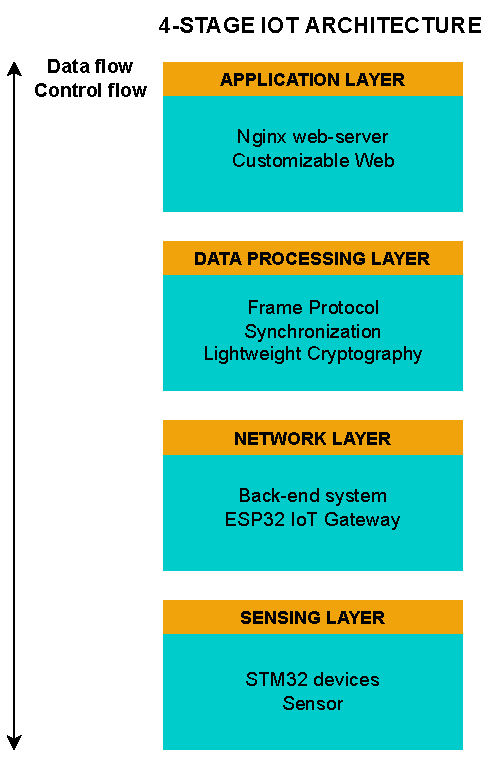
\includegraphics[width=8 cm]{images/Thesis-Page-2-IoT-Archi.pdf}
\caption{Mô hình 4 lớp của hệ thống IoT. Nguồn tham khảo InterviewBit~\cite{IoT-4-Layer-Archi}}
\label{fig:IoT-4-Layer-Archi}
\end{figure}

\begin{figure}[htp]
\centering
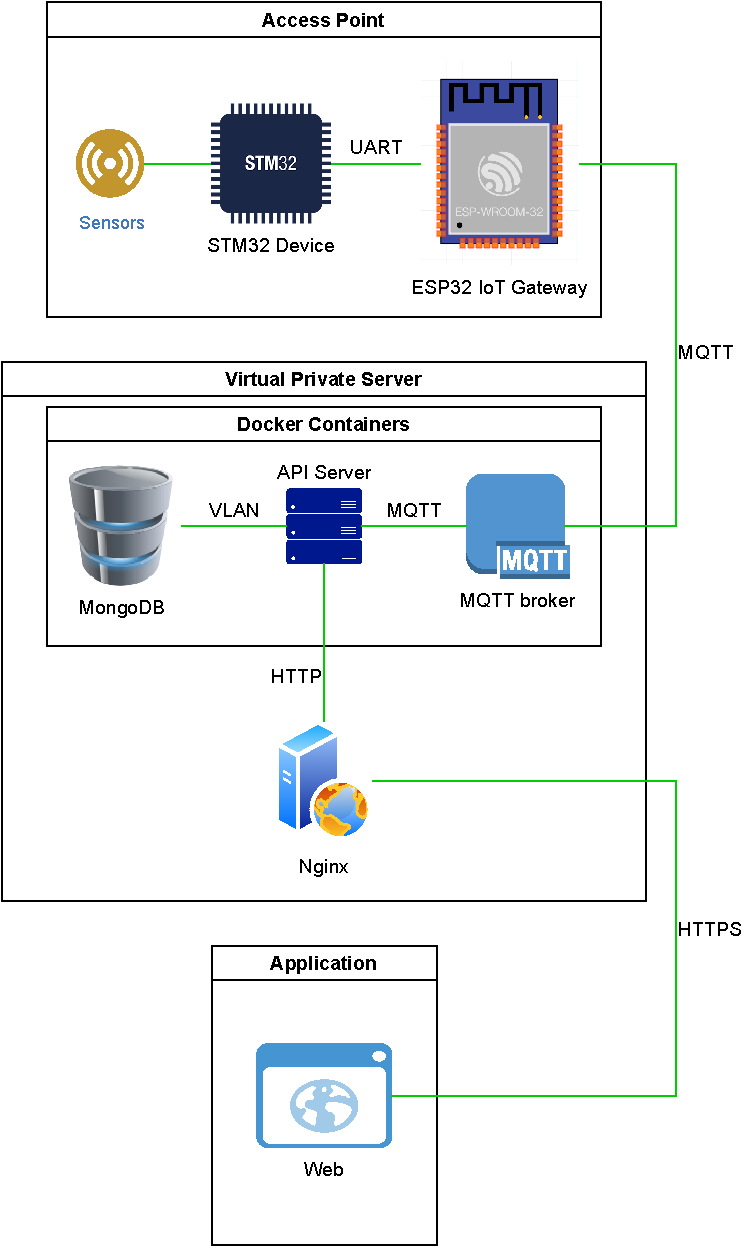
\includegraphics[width=0.75\linewidth]{images/Thesis-Page-3-IoT-Connections-Model.pdf}
\caption{Mô hình kết nối và giao thức của hệ thống IoT.}
\label{fig:IoT-Connections-Model}
\end{figure}

\section{Đóng góp}

% Đóng góp của nghiên cứu/ứng dụng của bạn?
    % Triển khai kỹ thuật giao tiếp và đồng bộ ở thiết bị STM32, gateway ESP32, và API server.
    % Triển khai kỹ thuật mật mã hóa nhẹ ChaCha20-Poly1305 trên gateway ESP32 và API server.
    % Phát triển hệ thống back-end và giao diện web.
    % Sử dụng kỹ thuật docker containerizing triển khai hệ thống back-end và nginx web-server cung cấp giao diện web
Kết quả của khóa luận này là những đóng góp trong kỹ thuật giao tiếp-đồng bộ, phát triển và triển khai hệ thống back-end và giao diện web. Trong giao tiếp-đồng bộ, kỹ thuật giao tiếp-đồng bộ đã được triển khai trên thiết bị STM32, gateway ESP32, và \acrshort{api} server. Trong mật mã hóa, kỹ thuật mật mã hóa nhẹ ChaCha20-Poly1305 đã áp dụng trên giao tiếp giữa gateway ESP32 và \acrshort{api} server. Trên hệ thống back-end, \acrshort{mqtt} broker và \acrshort{api} server được phát triển trên nền tảng NodeJS. Hơn nữa, kỹ thuật Docker containerizing được sử dụng để triển khai các thành phần của hệ thống back-end. Cuối cùng, về giao diện, giao diện được phát triển trên nền tảng Ant Design Pro và ngôn ngữ TypeScript, và được triển khai bằng máy chủ web Nginx.

\section{Bố cục}

%Tóm tắt luận văn được trình bày nhiều nhất trong 24 trang in trên hai mặt giấy, cỡ chữ Times New Roman 11 của hệ soạn thảo Winword hoặc phần mềm soạn thảo Latex đối với các chuyên ngành thuộc ngành Toán.

%Mật độ chữ bình thường, không được nén hoặc kéo dãn khoảng cách giữa các chữ.
%Chế độ dãn dòng là Exactly 17pt.
%Lề trên, lề dưới, lề trái, lề phải đều là 1.5 cm.
%Các bảng biểu trình bày theo chiều ngang khổ giấy thì đầu bảng là lề trái của trang.
%Tóm tắt luận án phải phản ảnh trung thực kết cấu, bố cục và nội dung của luận án, phải ghi đầy đủ toàn văn kết luận của luận án.
%Mẫu trình bày trang bìa của tóm tắt luận văn (phụ lục 1).

\chapter{CÁC HỆ THỐNG VÀ CÔNG NGHỆ LIÊN QUAN}
\label{Chapter2}

\section{Hệ thống IoT sử dụng nền tảng Blynk}

\subsection{Tổng quan về Blynk}

Blynk là một trong những nền tảng \acrshort{iot} được sử dụng nhiều nhất hiện nay. Nền tảng này cung cấp bộ ứng dụng toàn diện cho các hệ thống \acrshort{iot} của cá nhân, người dùng, và doanh nghiệp. Trên nền nảng này, bộ ứng dụng toàn diện của Blynk cho phép tạo mẫu (prototyping), phát triển, và quản lý từ xa các thiết bị điện tử được kết nối của tất cả phạm vi (scale)~\cite{Blynk-Overview}.

\subsection{Những vấn đề có thể giải quyết thông qua nền tảng Blynk}

% Những gì Blynk có thể cung cấp cho việc giải quyết bài toán BTS
Trong việc giám sát \acrshort{bts}, thiết kế, và triển khai hệ thống \acrshort{iot}, Blynk cung cấp giải pháp cho phần cứng, cấu hình, và giao diện.

    % Giải pháp bo mạch phần cứng.
Tại phần cứng, Blynk Library thư viện portable C++ dễ sử dụng và có thể chạy trên nhiều bo mạch. Cụ thể, thư viện này có thể cài đặt trên ESP32 \acrshort{iot} gateway của bo mạch của \acrshort{ptn} DESLab. Hơn nữa, Blynk Library dễ dàng cấu hình khi sử dụng Blynk Edgent. Đây là giải pháp được thiết kế để đơn giản hóa các kết nối của các thiết bị tới Blynk cloud. Vì vậy, Blynk Library và Edgent là những giải pháp phần cứng để triển khai giao thức kết nối tới cloud trên bo mạch.

    % Giải pháp cấu hình
Về mặt cấu hình, Blynk Console là ứng dụng web nhiều tính năng phục vụ cho nhiều đối tượng người dùng. Ứng dụng này cung cấp các template có sẵn để giúp người dùng dễ dàng cấu hình như General Setting, Datastream, Event, Notification, ... Dựa trên ứng dụng web Blynk Console, người dùng dễ dàng cấu hình các kênh dữ liệu cũng như kiểu dữ liệu của các Datastream. Từ đó, các cấu hình này tạo ra cơ sở dữ liệu lưu trữ các giá trị từ phần cứng và trực quan hóa các dữ liệu.

    % Giải pháp giao diện
Về mặt giao diện, nên tảng Blynk hỗ trợ người dùng giám sát và điều khiển các thiết bị trên dashboard trên nền tảng web và mobile app. Dựa trên các dashboard, người dùng có thể dễ dàng quản lý, quan sát dữ liệu từ thiết bị. Hơn nữa, đây là giao diện của no-code mobile app và web app, nên người dùng dễ dàng chỉnh sửa các widget trên giao diện hiển thị. Với các đặc tính của Blynk no-code editor, dashboard của hệ thống rất dễ dàng được thiết kế cho người dùng.

\subsection{Vấn đề không thể giải quyết thông qua Blynk}

% ko thể triển khai mật mã hóa trên cloud
Khi sử dụng Blynk, nền tảng này không cung cấp mã nguồn mở. Vì vậy, mật mã hóa không thể cài đặt trên giao tiếp giữa gateway và cloud. Đây là vấn đề lớn nhất dẫn đến việc hệ thống \acrshort{iot} không thể triển khai thông qua Blynk.

\section{Hệ thống IoT sử dụng ThingsBoard}

\subsection{Tổng quan về ThingsBoard}

ThingsBoard là một nền tảng \acrshort{iot} mã nguồn mở cho phép nhanh chóng phát triển, quản lý, và mở rộng của các dự án \acrshort{iot} \cite{ThingsBoard-Def-Overview}. Mục đích của ThingsBoard là cung cấp \acrshort{iot} cloud hoặc giải pháp tại chỗ (on-premises) một cách đột phá mà có thể cung cấp hạ tầng phía server cho các ứng dụng \acrshort{iot}.

\subsection{Những vấn đề có thể giải quyết thông qua nền tảng ThingsBoard}

Trong việc giám sát \acrshort{bts}, thiết kế, và triển khai hệ thống \acrshort{iot}, nền tảng ThingsBoard đưa ra giải pháp cho phần cứng, cấu hình, và giao diện.

Tại phần cứng, ThingsBoard Devices Library là tập hợp những hướng dẫn và đoạn code mà giải thích cách thức kết nối các \acrshort{iot} development board phổ biến tới nền tảng ThingsBoard \cite{ThingsBoard-Devices-Lib-Overview}. Trên hệ thống \acrshort{iot} được đề xuất, gateway ESP32 có thể sử dụng thư viện C++ ``Arduino ThingsBoard SDK''. Thư viện này giúp gateway ESP32 có thể tương tác với ThingsBoard cloud thông qua các giao thức như \acrshort{mqtt}, \acrfull{http}...

Về cấu hình, ThingsBoard web cho phép người dùng cấu hình các thiết bị trên trang ``Entities $\rightarrow$ Devices''. Từ đó, các thiết bị phần cứng có thể trao đổi dữ liệu với ThingsBoard cloud thông qua ``Access Token''.

Về giao diện, ThingsBoard web cho phép người dùng tạo các dashboard linh hoạt trên trang ``Dashboards''. Trên trang này, người dùng có thể chọn các widget để hiển thị các giá trị của bo mạch phần cứng.

\subsection{Vấn đề ThingsBoard không thể giải quyết}

Khác với Blynk, ThingsBoard là nền tảng \acrshort{iot} mã nguồn mở cung cấp giải pháp hạ tầng phía server. Vì vậy, hệ thống \acrshort{iot} được đề xuất, có thể host và tùy chỉnh ThingsBoard server trên \acrshort{vps}. Điều này có thể giúp hệ thống \acrshort{iot} cài đặt kỹ thuật mật mã hóa tùy chỉnh trên ThingsBoard server. Tuy nhiên, kích thước mã nguồn của ThingsBoad server là quá lớn và \acrshort{vps} của các quản trị viên không thể host ứng dụng server này. Vì vậy, kích thước mã nguồn quá lớn so với khả năng của \acrshort{vps} là nguyên nhân không thể sử dụng ThingsBoard server trên hệ thống \acrshort{iot}.

\section{Các hệ thống IoT đơn giản sử dụng ESP32 web server chế độ Access~Point}

\subsection{Những vấn đề có thể giải quyết khi sử dụng ESP32 web server chế độ Access Point}

Trong việc giám sát \acrshort{bts}, thiết kế, và triển khai hệ thống \acrshort{iot}, việc sử dụng ESP32 web server chế độ Access Point, có thể giải quyết vấn đề phần cứng, thiết kế, và triển khai hệ thống \acrshort{iot} tại một \acrshort{bts}.

Về phần cứng, \acrshort{mcu} ESP32 có thể được lập trình như một thiết bị và web server. Cụ thể, \acrshort{mcu} ESP32 có thể giao tiếp với các ngoại vi và cảm biến thông qua các \acrfull{gpio}.

Về cấu hình, hệ thống dựa trên mô hình này, chỉ sử dụng \acrshort{mcu} ESP32. Do đó, \acrshort{mcu} ESP32 có thể được cấu hình cơ sở dữ liệu một cách thủ công và triển khai kỹ thuật mật mã hóa nhẹ bằng việc lập trình firmware đơn thuần.

Về giao diện, \acrshort{mcu} ESP32 được cấu hình như một web server. Do đó, \acrshort{mcu} này cung cấp một giao diện tĩnh hiển thị các tương tác phục vụ cho việc hiển thị và điều khiển các giá trị trên cơ sở dữ liệu của nó.

\subsection{Những vấn đề không thể giải quyết khi sử dụng ESP32 web~server chế độ Access~Point}

Hệ thống \acrshort{iot} sử dụng ESP32 web server chế độ Access Point không thể giải quyết vấn đề kích thước hệ thống và giám sát hệ thống từ xa.

Đầu tiên, về vấn đề kích thước hệ thống, các quản trị viên \acrshort{vnpt} muốn giám sát nhiều \acrshort{bts} một cách tập trung. Khi đó, một \acrshort{mcu} ESP32 không đủ dung lượng để lưu trữ dữ liệu từ nhiều \acrshort{bts} cũng như dữ liệu người dùng.

Cuối cùng, khi sử dụng mô hình ESP32 web server, người dùng chỉ có thể truy cập giao diện web khi có cùng Access Point với \acrshort{mcu} ESP32. Vì vậy, khi người dùng giám sát từ xa và không có cùng Access Point với ESP32, người dùng không thể giám sát thông số của các \acrshort{bts}.

% Viết về lý thuyết của mô hình đang áp dụng trong việc giải quyết việc giám sát BTS.
% Đã chạy và thử nghiệm tại BTS
% Khó tiếp tục phát triển trong thời gian dài vì ko có các kỹ thuật cốt lõi.
% Cần có giao thức giao tiếp, cơ chế đồng bộ, giao diện tùy chỉnh, và cách thức triển khai mật mã hóa rõ ràng.
% viết về mô hình hệ thống iot sử dụng bo mạch phần cứng của PTN DESLab và máy chủ ảo
\section{Mô hình hệ thống IoT sử dụng bo mạch của PTN DESLab giao tiếp với VPS}

Đây là mô hình hệ thống \acrshort{iot} được áp dụng để giám sát các trạm \acrshort{bts}. Tại \acrshort{ptn} DESLab, mô hình này đã có kết quả để chạy và thử nghiệm trong thời gian ngắn hạn tại \acrshort{bts} của các quản trị viên \acrshort{vnpt}. Tuy nhiên, mô hình này vẫn phải đưa ra các khái niệm và kỹ thuật cốt lõi để có thể phát triển lâu dài. Trong khóa luận tốt nghiệp này, các khái niệm và kỹ thuật cốt lõi cần có, sẽ được trình bày và xây dựng để hệ thống \acrshort{iot} hiện tại, có thể tiếp tục phát triển. Các khái niệm cỗi lõi bao gồm mô hình-sơ đồ của hệ thống \acrshort{iot}, giao thức frame, cơ chế đồng bộ, cách thức triển khai mật mã hóa, và cách thức triển khai hệ thống back-end và giao diện.

\subsection{Mô hình và sơ đồ của hệ thống IoT}
\label{Model-Diagram-IoT-System}

Mô hình của hệ thống \acrshort{iot} cần được xây dựng, là mô hình \acrshort{iot} 4 lớp (minh họa như hình \ref{fig:IoT-4-Layer-Archi-C2}. Cụ thể, mô hình bao gồm sensing layer, network layer, data processing layer, và application layer.

\begin{figure}[htp]
\centering
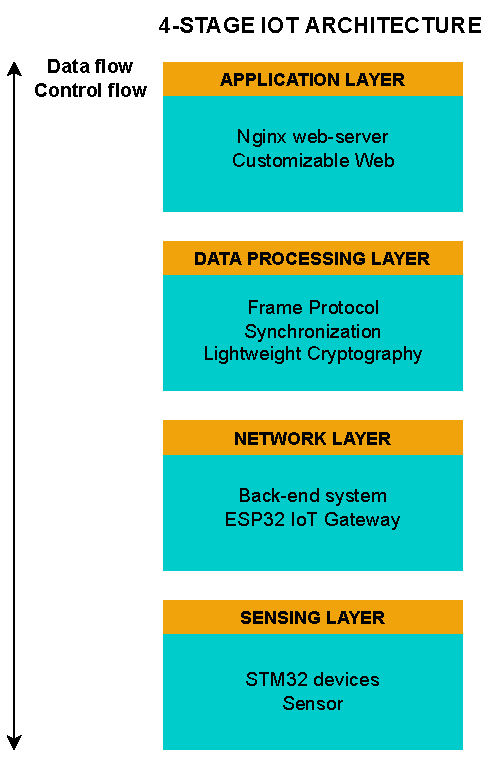
\includegraphics[width=8 cm]{images/Thesis-Page-2-IoT-Archi.pdf}
\caption{Mô hình 4 lớp của hệ thống IoT. Nguồn tham khảo InterviewBit~\cite{IoT-4-Layer-Archi}}
\label{fig:IoT-4-Layer-Archi-C2}
\end{figure}

\subsubsection{Sensing layer}

Đây là lớp đầu tiên của hệ thống \acrshort{iot} và sensing layer chứa các thiết bị vật lý, cảm biến, và ngoại vi trên bo mạch. Hoạt động của tầng này chủ yếu là thu thập và xử lý dữ liệu từ các cảm biến và ngoại vi, sau đó gửi dữ liệu lên tầng network.

Trong sensing layer, thiết bị sử dụng để giao tiếp với cảm biến và ngoại vi, là \acrshort{mcu} STM32. Các giao thức sử dụng trong tầng này là các giao thức có dây như UART, SPI, I2C,...

\subsubsection{Network layer}

Network layer là lớp chứa các thiết bị thu nhận và truyền tải dữ liệu trên Internet. Dựa trên lớp này, dữ liệu sẽ được luân chuyển từ \acrshort{iot} gateway đến các ứng dụng back-end.

Trong network layer, \acrshort{iot} gateway là \acrshort{mcu} ESP32 trên bo mạch. Gateway sẽ định tuyến dữ liệu từ hệ thống back-end đến sensing layer và ngược lại. Cuối cùng, hệ thống back-end thu nhận, xử lý, và lưu trữ dữ liệu từ sensing layer và đồng bộ các dữ liệu này với cơ sở dữ liệu của thiết bị vật lý và giao diện người dùng.

\subsubsection{Data processing layer}

Data processing layer là lớp chứa các kỹ thuật xử lý dữ liệu. Trong hệ thống này, data processing layer sẽ phân giải frame, mã hóa/giải mã dữ liệu, và đồng bộ dữ liệu với sensing và application layer.

\subsubsection{Application layer}

Application layer là lớp cung cấp ứng dụng của hệ thống thông qua các tương tác người dùng. Tại lớp này, hệ thống \acrshort{iot} sẽ cung cấp giao diện web tùy chỉnh cho người dùng. Từ đó, người dùng có thể giám sát và điều khiển dữ liệu của sensing và network layer.

\subsection{Giao thức frame}
\label{Frame-Protocol-subsec}

\subsubsection{Tổng quan về giao thức frame}

Giao thức frame được định nghĩa để tạo ra cấu trúc frame trong giao tiếp device-gateway. Cấu trúc frame này là duy nhất và khác biết với các hệ thống khác. Điều này giúp việc giao tiếp trên bo mạch dễ triển khai và có tính bảo mật.

% Tại sao sử dụng gia thức frame
Trên bo mạch, giao thức frame giúp giao tiếp device-gateway có tính bảo mật và đáng tin cậy. Đầu tiên, hệ thống sẽ có cấu trúc frame duy nhất, riêng tư, và bảo mật. Vì vậy, cấu trúc frame này không thể phân giải trên các hệ thống khác. Tiếp theo, vì giao tiếp device-gateway có thể bị lỗi do nhiễu trên bo mạch, nên cấu trúc frame cung cấp các byte CRC để phát hiện lỗi khi giao tiếp diễn ra. Điều này đảm bảo hệ thống vẫn hoạt động khi phát sinh lỗi trong giao tiếp device-gateway.

% Cấu trúc frame
\subsubsection{Cấu trúc frame}

Cấu trúc frame (minh họa như hình \ref{fig:Frame-Structure-Overview}) được thiết kế bằng cách bố trí thêm các byte header, trailer, và CRC vào dữ liệu truyền. Cụ thể, headers chứa 2-byte h1 và h2; trailers chứa 2-byte t1 và t2; CRC chứa 2-byte CRC1 và CRC2 để tính toán CRC 16-bit; và phần body chứa 1-byte command, 2-byte data length, và các byte data.

% Ý nghĩa của các byte
Để nhận diện frame, các header và trailer dùng để nhận diện phần đầu và cuối frame. Tiếp theo, 1-byte command, 2-byte data length, và các byte data để hệ thống thực thi lệnh với dữ liệu tương ứng của frame. Cuối cùng, 2-byte CRC dùng để soát lỗi trên phần body của frame.

\begin{figure}[htp]
\centering
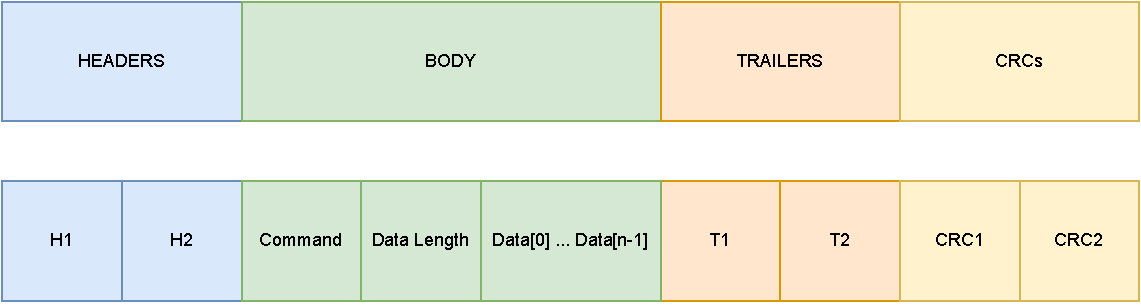
\includegraphics[width=0.9\linewidth]{images/Thesis-Page-4-Frame-Structure-Overview.pdf}
\caption{Cấu trúc frame của hệ thống.}
\label{fig:Frame-Structure-Overview}
\end{figure}

% Kỹ thuật phân giải frame

Để phân giải frame, kỹ thuật phân giải frame (minh họa như hình \ref{fig:frame-parsing-tech}) được triển khai trên giao tiếp UART của \acrshort{mcu} STM32 và gateway ESP32. Với mỗi byte nhận được, chỉ số của frame sẽ được kiểm tra. Với mỗi chỉ số frame, frame sẽ được kiểm tra header, trailer, CRC, hoặc thu thập các dữ liệu phần body. Cuối cùng, quá trình phần giải thành công khi việc kiểm tra các header, trailer và tính toán CRC thành công và quá trình thất bại khi việc kiểm tra header, trailer, và CRC thất bại; hoặc timeout.

\begin{figure}[htp]
\centering
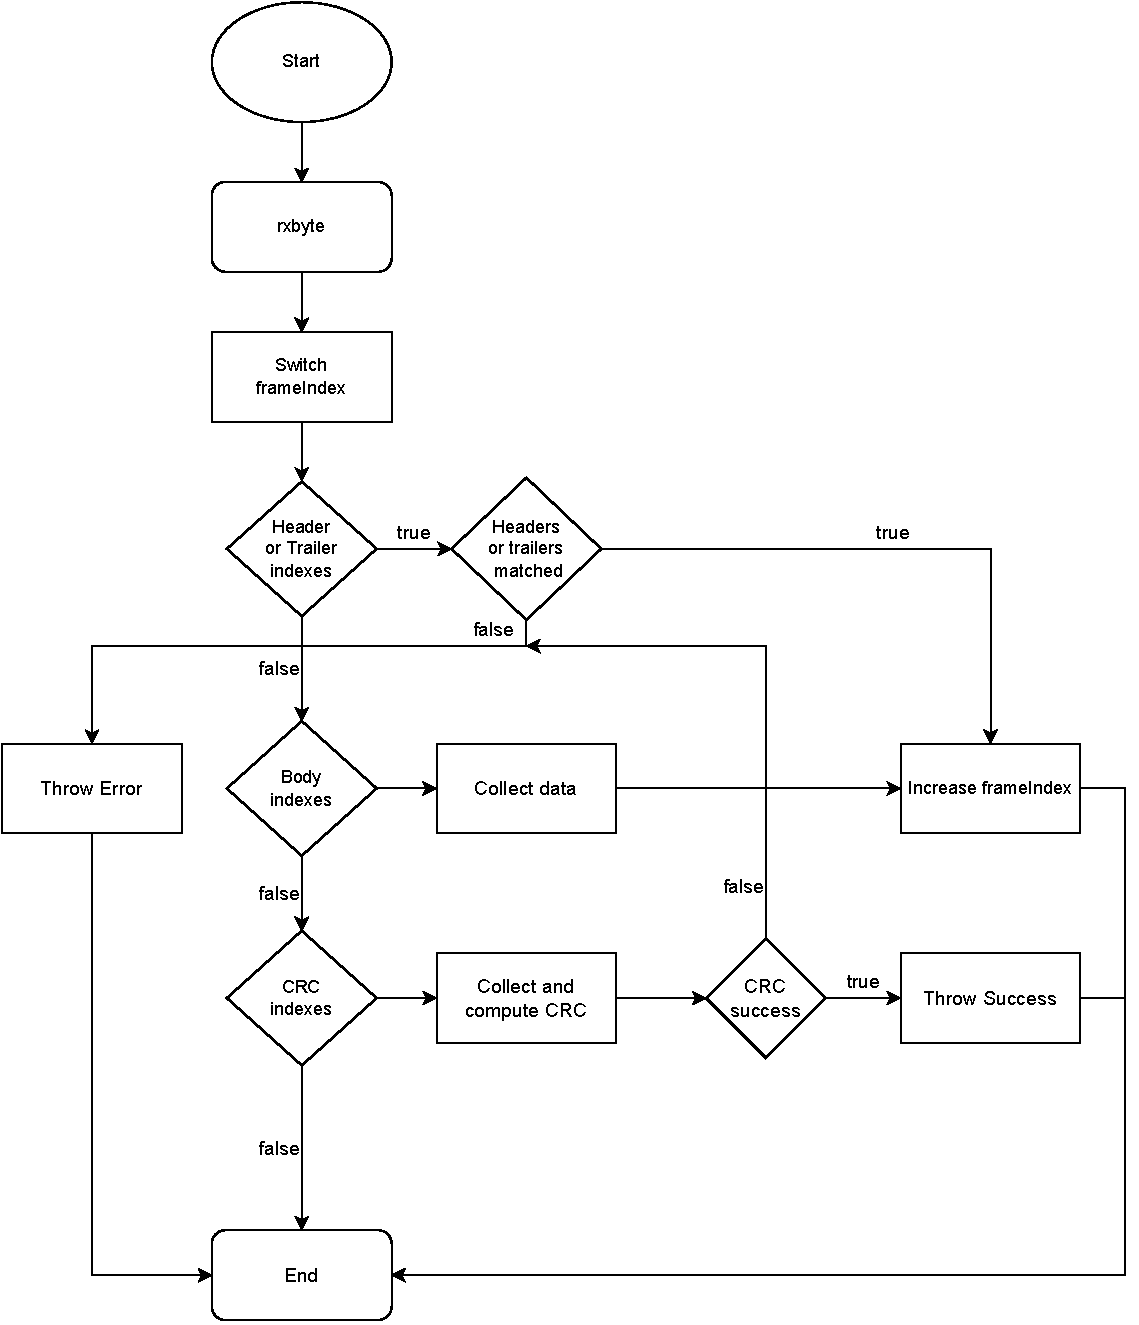
\includegraphics[width=1.0\linewidth]{images/Thesis-Page-5-Frame-Parsing-Tech.pdf}
\caption{Flowchart minh họa kỹ thuật phân giải frame.}
\label{fig:frame-parsing-tech}
\end{figure}

\subsection{Cơ chế đồng bộ}
\label{VSync-Mecha}

% Vì sao cần cơ chế đồng bộ
Cơ chế đồng bộ (minh họa như hình \ref{fig:sync-mechani-overview}) được thiết kế dựa trên các yêu cầu cập nhật database. Với mỗi yêu cầu cập nhật dữ liệu của database, database phải thông báo sự kiện cập nhật tới \acrshort{api} server. Thông qua sự kiện cập nhật từ database, \acrshort{api} server sẽ đồng bộ dữ liệu được cập nhật với bo mạch và giao diện. Giao diện sẽ được đồng bộ trực tiếp qua Internet và thiết bị được đồng bộ gián tiếp qua \acrshort{iot} gateway.

Trên hệ thống hiện tại, model của các \acrfull{vs} sẽ được đồng bộ khi có sự thay đổi dữ liệu của model này trên database. Khi có sự thay đổi dữ liệu model của \acrshort{vs}, dữ liệu model của \acrshort{vs} sẽ được đồng bộ tới thiết bị và giao diện thông qua cách thức hoạt động của cơ chế đồng bộ được đề cập.

\begin{figure}[htp]
\centering
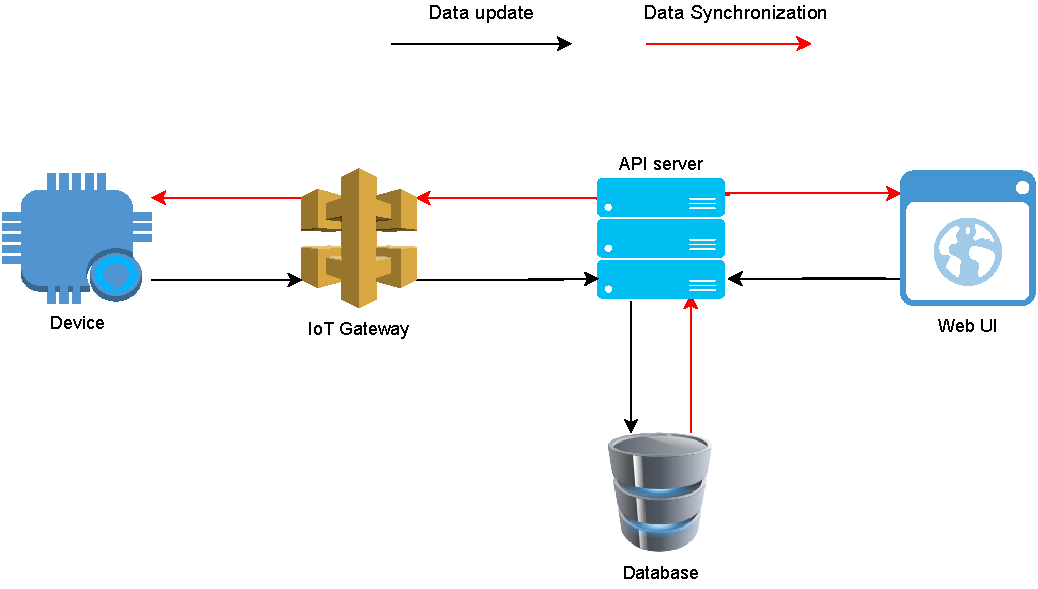
\includegraphics[width=1.0\linewidth]{images/Thesis-Page-6-sync-mecha.pdf}
\caption{Cơ chế đồng bộ của hệ thống \acrshort{iot}.}
\label{fig:sync-mechani-overview}
\end{figure}

\subsection{Giao diện web linh hoạt}

% Vì sao cần giao diện web linh hoạt
Trong các hệ thống \acrshort{iot}, cấu hình của các thiết bị luôn có thể thay đổi. Vì vậy, giao diện hiển thị cũng phải có tính linh hoạt và có thể tùy chỉnh để đáp ứng các thay đổi đó. Như vậy, giao diện có thể thay đổi tương ứng với cấu hình của các thiết bị. Hơn nữa, đối với người dùng, người dùng có thể dễ dàng thay đổi giao diện trong khi họ không cần phải lập trình.

% Cơ sở cho việc lập trình giao diện web linh hoạt
Giao diện web linh hoạt của hệ thống được phát triển trên framework ReactJS. Dựa trên framework này, thư viện ``React-Grid-Layout'' sẽ được sử dụng để phát triển giao diện linh hoạt. Khi sử dụng thư viện này, một hệ thống layout dạng lưới (minh họa như hình \ref{fig:RGL-overview}) sẽ được tạo ra. Trên mạng lưới đó, người dùng có thể kéo thả và thay đổi kích thước của các widget.

\begin{figure}[htp]
\centering
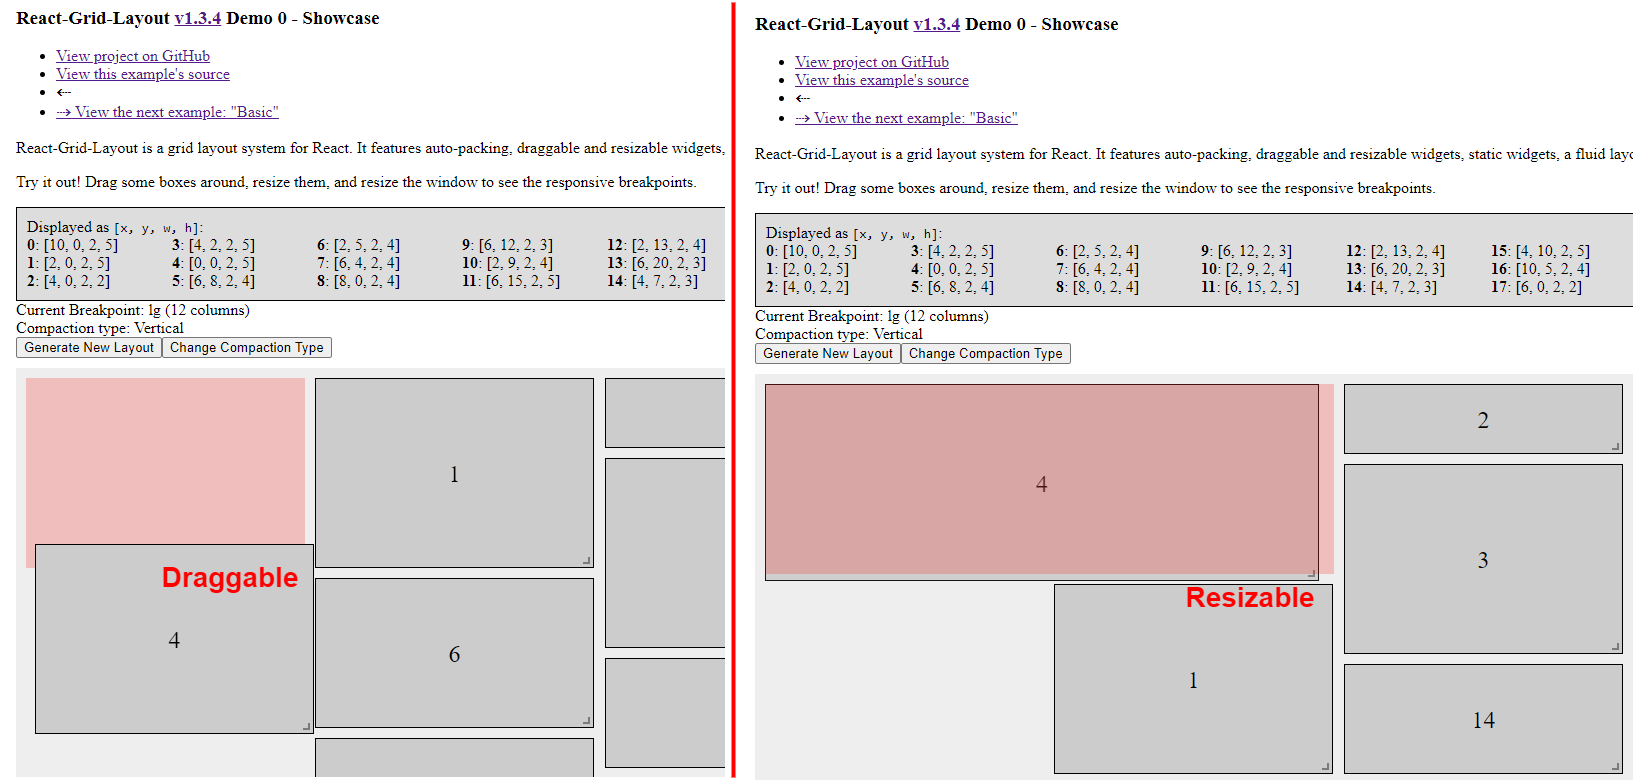
\includegraphics[width=1.0\linewidth]{images/Thesis-Page-7-RGL-Overview.png}
\caption{Hệ thống layout dạng lưới của React-Grid-Layout.}
\label{fig:RGL-overview}
\end{figure}

\subsection{Mật mã hóa nhẹ ChaCha20-Poly1305}

Mục này sẽ trích xuất và dịch thuật nội dung của RFC 7359~\cite{rfc7539}.

ChaCha20-Poly1305 là mật mã hóa xác thực với dữ liệu liên kết \acrfull{aead}. Đây là sự kết hợp của hai thuật toán độc lập. Thuật toán đầu tiên là ChaCha20, đây là thuật toán mã hóa dòng tốc độ cao. ChaCha20 được cho là nhanh hơn đáng kể so với thuật toán \acrfull{aes} trên môi trường software-only. Hơn nữa, ChaCha20 chạy nhanh hơn \acrshort{aes} ba lần trên những nền tảng không hỗ trợ phần cứng \acrshort{aes}. Về thuật toán Poly1305, Poly1305 là thuật toán xác thực tin nhắn tốc độ cao (high-speed message authentication code). Việc triển khai thuật toán này cũng rất dễ dàng và có độ chính xác cao.

\subsubsection{ChaCha Quarter Round}

Phép tính cơ bản của thuật toán ChaCha là quarter round. Nó tính toán dựa trên 4 số nguyên không dấu 32-bit, ký hiệu là a, b, c, và d. Việc tính toán diễn ra tuần tự như sau:

\begin{enumerate}
    \item a += b; d $\wedge$= a; d $<<<$= 16;
    \item c += d; b $\wedge$= c; b $<<<$= 12;
    \item a += b; d $\wedge$= a; d $<<<$= 8;
    \item c += d; b $\wedge$= c; b $<<<$= 7;
\end{enumerate}

Trong đó, dấu ``+'' ký hiệu cho phép cộng modulo 32-bit, ``$\wedge$'' ký hiệu cho toán tử bit \acrfull{xor}, và ``$<<<$ n'' ký hiệu cho n-bit dịch vòng bên trái (left rotation).

Về ChaCha state, ChaCha state là tập hợp của 16 số nguyên không dấu 32-bit, được biểu diễn dưới dạng ma trận 4x4 (như bảng \ref{tab:CC20-State-Pos}). Vì vậy, với mỗi phép toán quarter round, phép toán chỉ được thực hiện trên 4 trong số 16 số nguyên của ChaCha state.

\begin{table}[ht]
\caption{Mô tả bố cục ChaCha state ở dạng ma trận.}

\label{tab:CC20-State-Pos}%
\begin{center}
\begin{tabular}{|c|c|c|c|}
\hline
0  & 1  & 2  & 3  \\ \hline
4  & 5  & 6  & 7  \\ \hline
8  & 9  & 10 & 11 \\ \hline
12 & 13 & 14 & 15 \\ \hline
\end{tabular}
\end{center}
\end{table}

\subsubsection{ChaCha20 Block Function}

ChaCha20 Block Function là quá trình thực hiện việc biến đổi một ChaCha state bằng việc thực hiện nhiều lần các quarter round.

Đầu vào của khối ChaCha20 bao gồm:
\begin{itemize}
    \item Một key 256-bit, là sự kết hợp của 8 số nguyên 32-bit little-endian.
    \item Một nonce 96-bit, là sự kết hợp của 3 số nguyên 32-bit little-endian.
    \item Một khối đếm (block count parameter), là một số nguyên 32-bit little-endian.
\end{itemize}

Đầu ra của khối là 64 byte ngẫu nhiên.

Về việc khởi tạo ChaCha State, ChaCha State được khởi tạo bằng cách bố trí các tham số đầu vào của ChaCha20 dưới dạng ma trận 4x4 (minh họa như bảng \ref{tab:Init-CC20-State}) như sau:

\begin{itemize}
    \item 4 word đầu tiên (từ vị trí 0$\rightarrow$3) là các constant: 0x61707865, 0x3320646e, 0x79622d32, 0x6b206574.
    \item 8 word tiếp theo (từ vị trí 4$\rightarrow$11) được trích xuất từ 256-bit key bằng việc đọc các byte theo trật tự little-endian, đọc theo từng khối, mỗi khối là 1 word.
    \item Word thứ 12 là block counter. Vì mỗi ChaCha Block có độ dài 64 byte, một word 32-bit đủ cho 256 gigabytes dữ liệu. % 2^32 (bit) / 64(byte) = 256 ggByte
    \item Các word thứ 13$\rightarrow$15 là nonce, cùng một key thì không nên lặp lại nonce. Word thứ 13 là 32 bit đầu tiên của đầu vào nonce như một số nguyên little-endian, trong khi đó, word thứ 15 là 32 bit còn lại.
\end{itemize}

\begin{table}[ht]
\caption{Ma trận khởi tạo của ChaCha state.}

\label{tab:Init-CC20-State}%
\begin{center}
\begin{tabular}{|c|c|c|c|}
\hline
cccccccc & cccccccc & cccccccc & cccccccc \\ \hline
kkkkkkkk & kkkkkkkk & kkkkkkkk & kkkkkkkk \\ \hline
kkkkkkkk & kkkkkkkk & kkkkkkkk & kkkkkkkk \\ \hline
bbbbbbbb & nnnnnnnn & nnnnnnnn & nnnnnnnn \\ \hline
\end{tabular}
\end{center}
\end{table}

Trong đó, c=constant, k=key, b=blockcount, và n=nonce

Trong ChaCha20 Block Function, ChaCha20 chạy 20 round, xen kẽ giữa ``column rounds'' và ``diagonal rounds''. Mỗi round bao gồm bốn quarter-round, được minh họa như trình tự bên dưới. Trong một round của ChaCha20 Block Function, các quarter-round 1$\rightarrow$4 là phần thuộc ``column'' round, và 5$\rightarrow$8 là phần thuộc ``diagonal'' round:

\begin{enumerate}
    \item QUARTERROUND(0, 4, 8, 12)
    \item QUARTERROUND(1, 5, 9, 13)
    \item QUARTERROUND(2, 6, 10, 14)
    \item QUARTERROUND(3, 7, 11, 15)
    \item QUARTERROUND(0, 5, 10, 15)
    \item QUARTERROUND(1, 6, 11, 12)
    \item QUARTERROUND(2, 7, 8, 13)
    \item QUARTERROUND(3, 4, 9, 14)
\end{enumerate}

Sau khi kết thúc 20 round (hoặc 10 lần thực hiện 8 trình tự ở trên), các word đầu vào ban đầu được cộng với các word đầu ra. Sau đó, kết qua được serialize bằng việc sắp xếp các từng word một theo trình tự little-endian.

\subsubsection{Thuật toán mã hóa ChaCha20}

ChaCha20 là mã hóa dòng được thiết kế bởi D. J. Bernstein. Nó là sự cải tiến của thuật toán Salsa20, và sử dụng 256-bit key.

ChaCha20 liên tục thực thi ChaCha20 Block Function, với cùng key và nonce, và với việc liên tục tăng block counter. Sau đó, ChaCha20 sẽ tuần tự hóa (serialize) kết quả của ChaCha state bằng việc ghi các số theo thứ tự little-endian, tạo keystream block.

Đầu vào của thuật toán ChaCha20 bao gồm
\begin{itemize}
    \item Một key 256-bit.
    \item Một counter 32-bit ban đầu. Counter có thể thiết lập bất cứ giá trị nào, nhưng thường là 0 hoặc 1. Điều này có nghĩa khi dùng một lần nếu ta sử dụng khối couter 0 cho việc gì đó, ví dụ như việc tạo ra one-time authenticator key như là một phần của thuật toán \acrshort{aead}.
    \item Một nonce 96-bit. Trong một số giao thức, nonce được xem như là một vector khởi tạo.
    \item Một plaintext có độ dài tùy ý.
\end{itemize}

Đầu ra của thuật toán là tin nhắn được mã hóa, hoặc ``ciphertext'', có cùng độ dài.

Việc giải mã được tiện hành tương tự như mã hóa. ChaCha20 Block Function được sử dụng để tạo keystream, nó được dùng để \acrshort{xor} với ciphertext để khôi phục lại plaintext.

\subsubsection{Thuật toán Poly1305}
\label{Poly1305Algorithm}

Poly1305 là thuật toán tạo xác thực một lần (one-time authenticator) được thiết kế bởi D. J. Bernstein. Poly1305 dùng 32-byte one-time key và một message, và cho ra một xác thực 16-byte tag. Tag này dùng để xác thực message.

Bất kể key được tạo ra như thế nào, key được phân vùng thành hai phần, được gọi là ``r'' và ``s''. Cặp (r,s) nên là duy nhất, và bắt buộc không thể dự đoán trước trong mỗi lần tạo, ``r'' có thể tùy chỉnh là một hằng số.

``s'' nên được tạo ra có tính chất không thể dự đoán trước, nhưng hoàn toàn chấp nhận việc tạo ra cả ``r'' và ``s'' một cách duy nhất tại một thời điểm. Bởi vì cả ``r'' và ``s'' đều có độ dài 128 bit, nên tạo ra chúng một cách ngẫu nhiên thì cũng chấp nhận được.

Đầu vào của thuật toán Poly1305 bao gồm:

\begin{itemize}
    \item Một one-time key 256-bit.
    \item Một message có độ dài tùy ý.
\end{itemize}

Đầu ra của thuật toán là 128-bit tag.

Thuật toán Poly1305 diễn ra tuần tự như sau. Đầu tiên, giá trị của ``r'' được kẹp chặt (clamp).

Tiếp đến, thiết lập hằng số nguyên số ``P'' là $2^{135}$ – 5: 3fffffffffffffffffffffffffffffffb. Sau đó ta cũng thiết lập biến ``accumulator'' bằng 0.

Sau đó, chia message thành các khối 16-byte. Khối cuối cùng có thể có độ dài ngắn hơn:

\begin{itemize}
    \item Đọc khối message như từng số little-endian.
    \item Thêm một bit ở vị trí ngoài cùng của các octet. Với một khối 16-byte, điều này tương đương với việc cộng với $2^{128}$. Khối có độ dài nhỏ hơn 10-byte, nó có thể là $2^{120}$, $2^{112}$, hoặc bất cứ số là lũy thừa của 2 mà nó có thể chia hết cho 8, nhỏ nhất là $2^8$.
    \item Nếu block không có độ dài 17 byte (ở block cuối cùng), thêm các bit 0 (pad) vào block. Điều này là vô nghĩa nếu ta coi các block như các số nguyên.
    \item Cộng số này với ``accumulator''.
    \item Nhân ``accumulator'' với ``r''.
    \item Thiết lập ``accumulator'' bằng phép chia modulo cho ``P''. \\Tóm lại: $accumumator = ((accumulator+block)*r) \% P$.
\end{itemize}

Cuối cùng, giá trị của secret key (``s'') được cộng vào ``accumulator'',  và 128 least significant bit được tuần tự hóa theo trật tự little-endian.

\subsubsection{Tạo Poly1305 key sử dụng ChaCha20}
\label{CreatePoly1305UsingChaCha20}

Như đã đề cập ở mục \ref{Poly1305Algorithm}, có thể chấp nhận việc tạo one-time key cho Poly1305 một cách giả ngẫu nhiên (pseudorandomly). Ở mục này, phương pháp được đề xuất là tạo one-time key cho Poly1305 sử dụng ChaCha20.

Để tạo cặp key (r,s), chúng ta sử dụng ChaCha20 Block Function. Phương pháp được đề xuất là gọi ChaCha20 Block Function với các tham số đầu vào như sau:

\begin{itemize}
    \item 256-bit key từ keystream sinh ra từ ChaCha20 Block Function.
    \item Block counter thiết lập bằng 0.
    \item Một nonce 96-bit.
\end{itemize}

Sau khi chạy ChaCha20 Block Function, nó sinh ra 512-bit state. Lấy 256 bit đầu tiên hoặc state tuần tự hóa (serialized state), và sử dụng chúng như one-time Poly1305 key: 128 bit đầu tiên giữ lại và hình thành nên ``r'', và 128 bit còn lại trở thành ``s''. 256 bit còn lại bị loại bỏ.

\subsubsection{Cấu trúc AEAD}

Cấu trúc \acrshort{aead} cho thuật toán ChaCha20-Poly1305 là mã hóa xác thực với dữ liệu liên kết. Các input cho AEAD\_CHACHA20\_POLY1305 là:

\begin{itemize}
    \item Một key 256-bit.
    \item Một nonce 96-bit.
    \item Một plaintext có độ dài tùy ý.
    \item Dữ liệu xác thực liên kết với độ dài tùy ý - \acrfull{aad}.
\end{itemize}

Các thuật toán gốc của ChaCha20 và Poly1305 được kết hợp thành \acrshort{aad} có đầu vào là một key 256-bit và nonce 96-bit như sau:

\begin{itemize}
    \item Đầu tiên, Poly1305 one-time key được tạo ra từ key 256-bit và nonce sử dụng phương pháp ở mục \ref{CreatePoly1305UsingChaCha20}.
    \item Tiếp theo, function, thực hiện mã hóa ChaCha20, được thực thi để mã hóa plaintext, sử dụng cùng key và nonce, và với couter được thiết lập bằng 1.
    \item Cuối cùng, Poly1305 function được thực thi với đầu vào là Poly1305 key được tính toán ở trên, và một message (plaintext).
\end{itemize}

Output từ \acrshort{aead} là hai thành phần sau:
\begin{itemize}
    \item Một ciphertext có cùng độ dài với plaintext.
    \item Một tag 128-bit, là output của Poly1305 function.
\end{itemize}

Việc giải mã là tương tự với những khác biệt sau:
\begin{itemize}
    \item Các vai trò của ciphertext và plaintext được hoán đổi, nên function mã hóa ChaCha20 được áp dụng cho ciphertext, cung cấp plaintext.
    \item Poly1305 function vẫn thực thi dựa trên \acrshort{aad} và cipher text, không phải plaintext.
    \item Tag được tạo ra, được so sánh tag nhận được. Message được xác thực khi và chỉ khi các tag trùng khớp với nhau.
\end{itemize}

\chapter{\tenKL}
\label{Chapter3}

% Dẫn nhập: mô tả chi tiết phương pháp thực hiện và giải pháp đề xuất trên mô hình, bo mạch, giao diện web, và hệ thống back-end
Chương \ref{Chapter3} mô tả chi tiết phương pháp thực hiện và giải pháp đề xuất trên mô hình hệ thống \acrshort{iot}. Các mô tả này bao gồm mô hình, bo mạch, giao diện web, và hệ thống back-end.

\section{Mô hình hệ thống IoT}

% Tổng quan về mô hình: phần cứng, máy chủ ảo.
Mô hình hệ thống \acrshort{iot} được đề xuất (minh họa như hình \ref{fig:IoT-Model-Overral}), được triển khai dựa trên sự kết hợp của bo mạch, hệ thống back-end, giao diện web, và giao thức kết nối giữa chúng. Dựa trên các thành phần này, mô hình \acrshort{iot} 4 lớp (được đề cập ở mục \ref{Model-Diagram-IoT-System}) sẽ được áp dụng. Trên mô hình này, bo mạch của \acrshort{ptn} DESLab và \acrshort{vps} của các quản trị viên \acrshort{vnpt} là hai thành phần chủ đạo.

Trên bo mạch, bo mạch được thiết kế dựa trên kết nối của các \acrshort{mcu} STM32 và ESP32. Trong đó, \acrshort{mcu} STM32 là thiết bị giao tiếp vạn vật (things) và thuộc sensing layer. Tiếp theo, \acrshort{mcu} ESP32 là \acrshort{iot} gateway định tuyến các luồng dữ liệu trong giao tiếp sensing-network layer và thuộc lớp network layer.

Trên \acrshort{vps}, hệ thống \acrshort{iot} triển khai hệ thống back-end và Nginx web server. Cụ thể, hệ thống back-end bao gồm \acrshort{mqtt} Broker, EggJS \acrshort{api} server, và MongoDB database. Cuối cùng, Nginx web server cung cấp giao diện người dùng và giao diện người dùng được phát triển trên nền tảng ReactJS và giải pháp Ant Design Pro.

Trên hệ thống \acrshort{iot}, hệ thống có 3 kỹ thuật xử lý dữ liệu. Đó là giao thức frame, mật mã hóa nhẹ ChaCha20-Poly1305, và đồng bộ. Trong đó, giao thức frame được triển khai trên thiết bị STM32, ESP32 gateway, và \acrshort{api} server. Tiếp theo, mật mã hóa ChaCha20-Poly1305 được sử dụng trên ESP32 gateway và \acrshort{api} server. Cuối cùng, cơ chế đồng bộ được triển khai trên \acrshort{api} server, giao diện web, và thiết bị STM32.

Về các giao thức truyền, hệ thống sử dụng giao thức có dây \acrfull{uart}; các giao thức không dây: \acrshort{mqtt}, \acrfull{https}, và Websocket; và \acrfull{vlan}. Trong đó, \acrshort{uart} được sử dụng trong giao tiếp gateway-device; \acrshort{mqtt} được sử dụng trong giao tiếp gateway-\acrshort{mqtt} Broker và \acrshort{mqtt} Broker-\acrshort{api} server; \acrshort{https} và Websocket được sử dụng trong giao tiếp \acrshort{api} server-web; và \acrshort{vlan} được sử dụng trong giao tiếp \acrshort{api}~server-database.

\begin{figure}[htp]
\centering
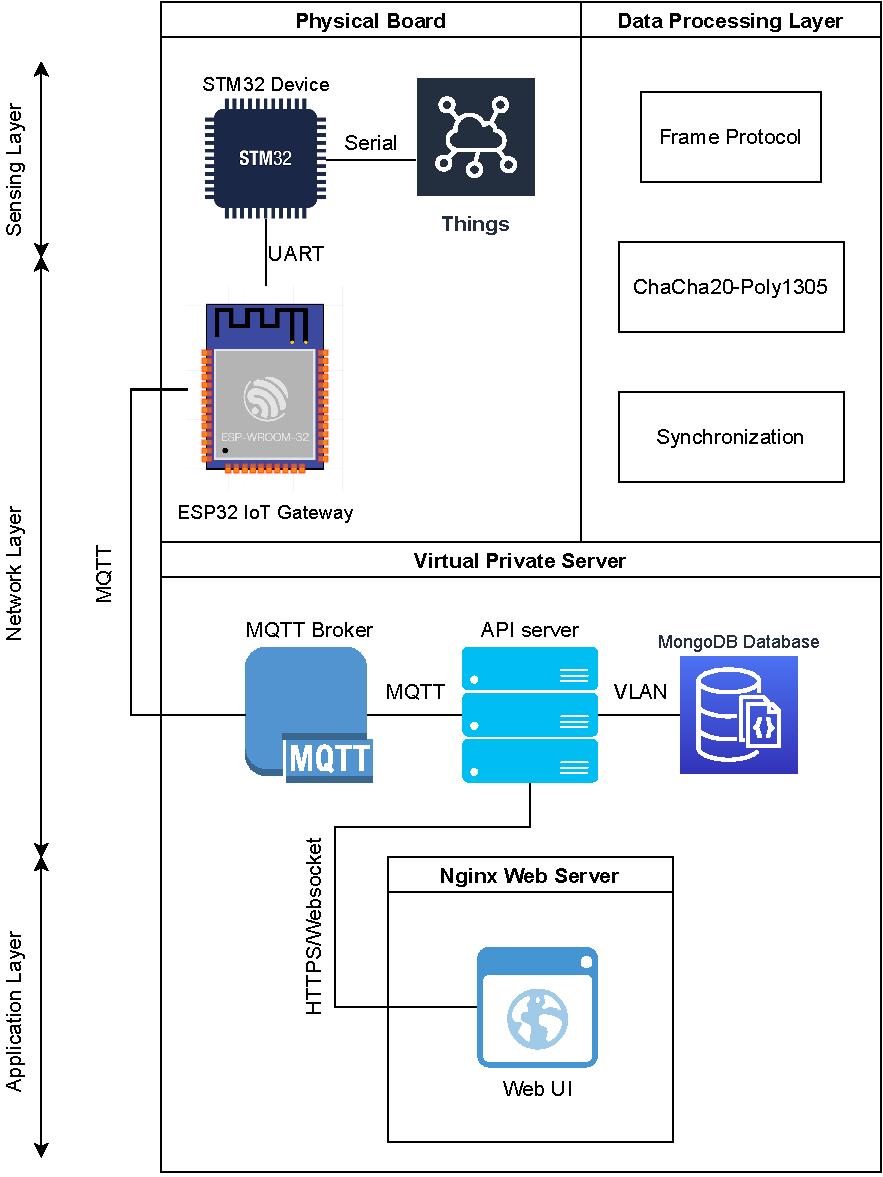
\includegraphics[width=1.0\linewidth]{images/Thesis-Page-8-IoT-Model-Overral.pdf}
\caption{Mô hình hệ thống \acrshort{iot} được đề xuất.}
\label{fig:IoT-Model-Overral}
\end{figure}

% Nội dung về bo mạch phát triển, các kỹ thuật trên bo mạch.
\section{Bo mạch phần cứng}

% Giới thiệu về bo mạch
Bo mạch phần cứng được sử dụng để xây dựng hệ thống \acrshort{iot} (minh họa ở hình \ref{fig:IoT-Dev-Board}), là bo mạch phát triển \acrshort{iot} của \acrshort{ptn} DESLab. Bo mạch này bố trí hai \acrshort{mcu} STM32F407VGT6 và ESP Wroom 32 kèm theo các ngoại vi. Các ngoại vi bao gồm led, nút nhấn, switch, màn hình OLED, và các \acrshort{gpio} của hai \acrshort{mcu}.

\begin{figure}[htp]
\centering
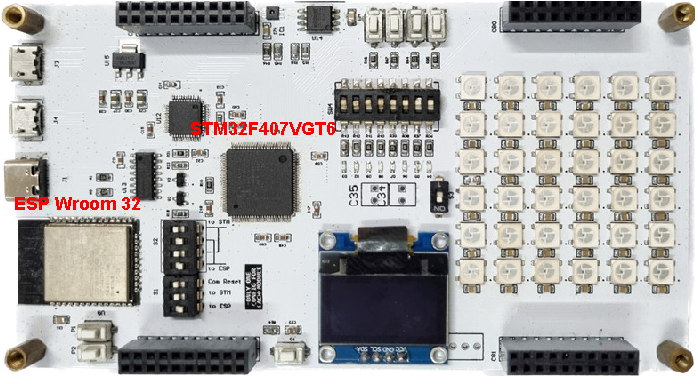
\includegraphics[width=1.0\linewidth]{images/Thesis-Page-1-Bo-mach.pdf}
\caption{Bo mạch phát triển \acrshort{iot} của \acrshort{ptn} DESLab.}
\label{fig:IoT-Dev-Board}
\end{figure}

% Chỉ trình bày chi tiết về chức năng của các MCU, ko giải thích source
\subsection{ESP32 IoT gateway}
\label{ESP32-IoT-gateway}

% Mục đích sử dụng, giới thiệu về các chức năng sẽ trình bày.
\acrshort{mcu} ESP32 được phát triển trên framework Arduino, platform PlatformIO, và ngôn ngữ C++. ESP32 được bố trí trên bo mạch phát triển và có sẵn module WiFi (Wi-Fi: 802.11 b/g/n/e/i, 2.5 GHz). Vì vậy, \acrshort{mcu} ESP32 được phát triển để được sử dụng như một \acrshort{iot} gateway. Về cơ bản, ESP32 \acrshort{iot} gateway có nhiệm vụ định tuyến các luồng dữ liệu trong giao tiếp STM32 device-\acrshort{api} server và ngược lại. Để thực hiện được công việc này, \acrshort{mcu} ESP32 phải thực hiện công việc phân giải và xử lý frame giao tiếp cũng như đệm dữ liệu (buffering data).

Về việc đệm dữ liệu, \acrshort{mcu} ESP32 sử dụng bộ đệm vòng (circular buffer) có kích thước cố định để lưu trữ tạm thời các dữ liệu nhận được. Trên bo mạch hiện tại, ESP32 có hai bộ đệm vòng để nhận dữ liệu qua giao tiếp \acrshort{uart} từ \acrshort{mcu} STM32 và qua giao tiếp \acrshort{mqtt} từ \acrshort{mqtt} Broker. Cụ thể, bộ đệm vòng UART nhận dữ liệu từ ngắt \acrshort{uart} và bộ đệm vòng \acrshort{mqtt} nhận dữ liệu từ \acrshort{mqtt} message callback. Dựa trên các buffer này, ESP32 tiến hành phân xử từng buffer (minh họa như hình \ref{fig:CBuf-Abritrating}) trong vòng lặp vô hạn của firmware. Để phân xử hợp lý cho từng bộ đệm, buffer selector được triển khai để lựa chọn buffer trong mỗi vòng lặp. Việc này giúp các buffer luôn được kiểm tra và mỗi buffer sẽ được tiến hành xý lý khi nó có dữ liệu.

\begin{figure}[htp]
\centering
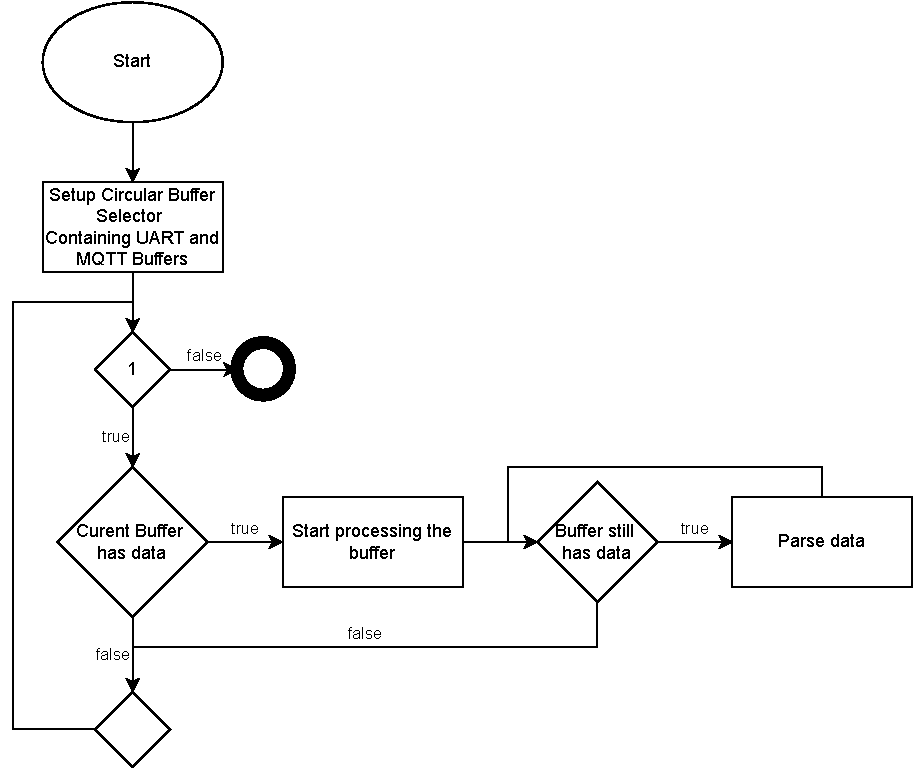
\includegraphics[width=1.0\linewidth]{images/Thesis-Page-9-CBuf-Abritrating.pdf}
\caption{Quá trình phân xử các bộ đệm vòng.}
\label{fig:CBuf-Abritrating}
\end{figure}

Về quá trình phân giải và xử lý frame, quá trình này diễn ra để xử lý dữ liệu trong bộ đệm vòng. Khi bộ đệm có dữ liệu, quá trình phân giải frame sẽ diễn ra trong một process độc lập (minh họa như hình \ref{fig:Frame-Parsing-Process}). Process này sẽ kết thúc khi frame được phân giải thành công, thất bại, hoặc timeout.

\begin{figure}[htp]
\centering
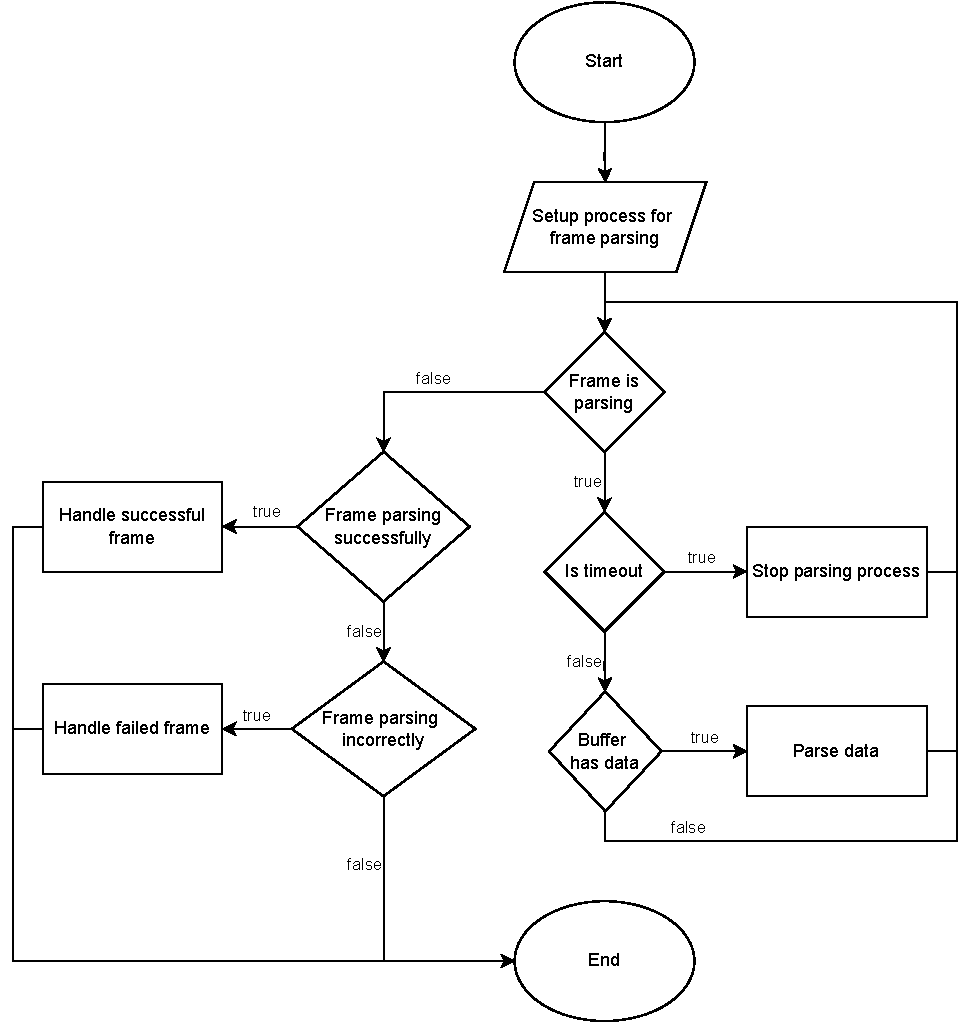
\includegraphics[width=1.0\linewidth]{images/Thesis-Page-10-Frame-Parsing-Process.pdf}
\caption{Process phân giải frame.}
\label{fig:Frame-Parsing-Process}
\end{figure}

\subsection{STM32 device}

\acrshort{mcu} STM32 được phát triển trên công cụ STM32CubeIDE và sử dụng ngôn ngữ C. STM32 được phát triển như một thiết bị vật lý trong mô hình \acrshort{iot}. Cụ thể, \acrshort{mcu} STM32 có nhiệm vụ tương tác với các cảm biến và ngoại vi cũng như đồng bộ dữ liệu với \acrshort{api} server.

STM32 thực hiện đệm dữ liệu, xử lý và phân giải frame như ESP32 gateway (được đề cập trong mục \ref{ESP32-IoT-gateway}). Ngoài ra, STM32 có thể đọc và thay đổi cơ sở dữ liệu trên \acrshort{vps} thông qua các \acrshort{api}. Các \acrshort{api} này giúp STM32 gửi yêu cầu đọc ghi dữ liệu và đồng bộ với cơ sở dữ liệu. Các \acrshort{api} này bao gồm \acrshort{api} đọc dữ liệu của \acrshort{vs}; và ghi dữ liệu \acrshort{vs} theo kiểu Integer và Float.

\section{Hệ thống back-end}

Hệ thống back-end là tập hợp những ứng dụng server chạy trên \acrshort{vps}. Những ứng dụng này bao gồm \acrshort{mqtt} Broker, \acrshort{api} server, và MongoDB database. Trên \acrshort{vps}, hệ thống back-end được triển khai bằng kỹ thuật Docker Containerizing.

\subsection{MQTT Broker}

\acrshort{mqtt} Broker, trung tâm của giao thức Publish/Subscribe \acrshort{mqtt}, là một ứng dụng server thu nhận tất cả các message từ các \acrshort{mqtt} client và định tuyến đến những subscribing client thích hợp \cite{MQTT-Broker-Def}.

Trong hệ thống \acrshort{iot} được đề xuất, \acrshort{mqtt} Broker được xây dựng trên framework NodeJS và ngôn ngữ JavaScript. Trong \acrshort{mqtt} Broker, các \acrshort{mqtt} client là \acrshort{iot} gateway và \acrshort{api} server. Hơn nữa, các dữ liệu publish/subscribe trên \acrshort{mqtt} Broker đều được mã hóa bởi thuật toán ChaCha20-Poly1305.

% Mô hình
Về tổ chức kết nối, giao thức \acrshort{mqtt} sử dụng các topic để quản lý luồng dữ liệu. Trên hệ thống \acrshort{iot}, các gateway và \acrshort{api} server sẽ được tổ chức kết nối \acrshort{mqtt} thông qua việc publish/subscribe (minh họa như hình \ref{fig:Frame-Parsing-Process-2}). Trong đó, \acrshort{api} server subscribe vào một topic và các gateway cùng gửi dữ liệu từ phần cứng vào cùng một topic đó. Trong khi, các gateway sẽ subscribe vào một topic riêng biệt và \acrshort{api} server gửi dữ liệu tới phần cứng thông qua từng topic riêng biệt đó. Các topic của gateway được phân biệt thông qua 12-byte gateway ID.

\begin{figure}[htp]
\centering
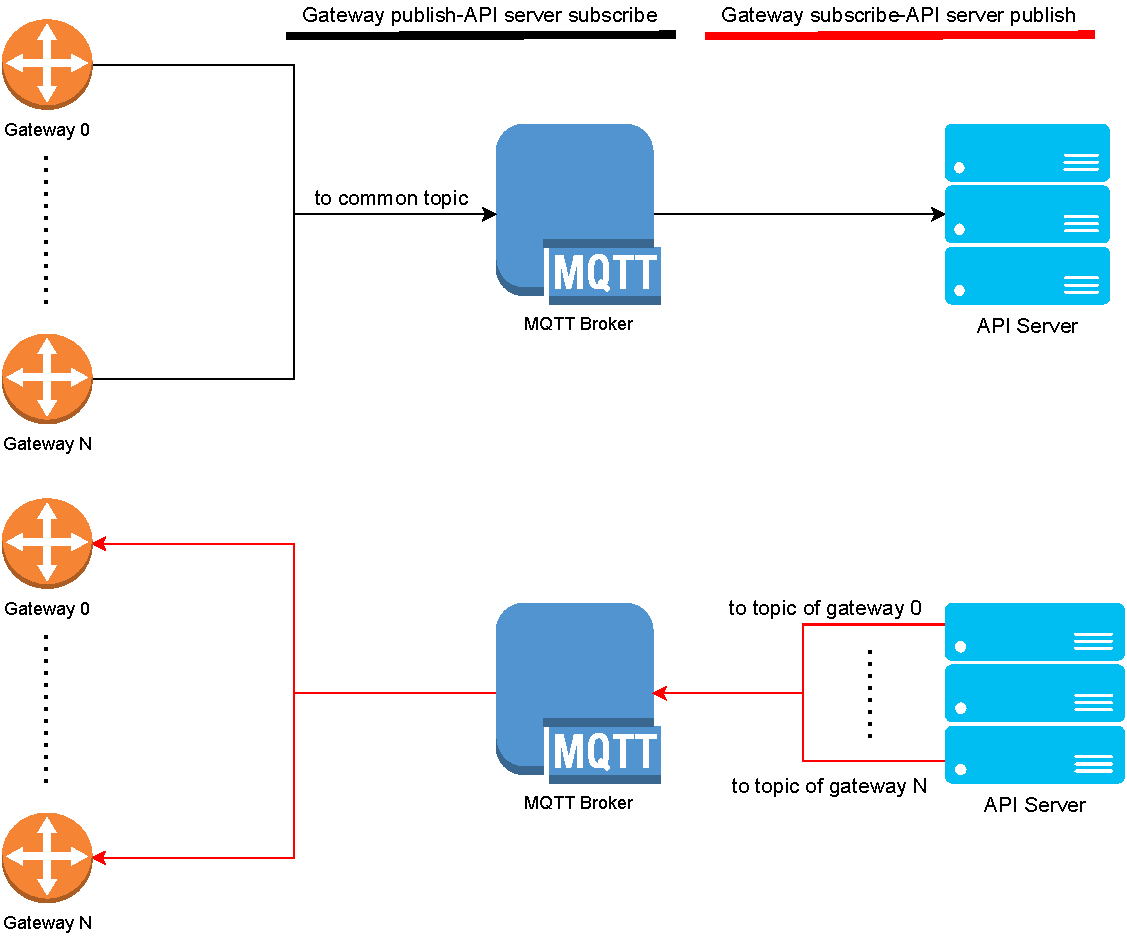
\includegraphics[width=1.0\linewidth]{images/Thesis-Page-11-MQTT-Connect-Establish.pdf}
\caption{Mô hình Publish/Subscribe MQTT trên hệ thống IoT.}
\label{fig:Frame-Parsing-Process-2}
\end{figure}

% Tổng quan, kết nối với thiết bị, kết nối với CSDL, và web.
\subsection{API Server}

\acrshort{api} server, trung tâm của hệ thống \acrshort{iot}, là ứng dụng server được xây dựng trên nền tảng EggJS, môi trường NodeJS, và ngôn ngữ JavaScript. Trên hệ thống, \acrshort{api} server có nhiệm vụ thu nhận và xử lý dữ liệu cũng như cung cấp dịch vụ truy xuất database cho phần cứng và giao diện web. Cụ thể, \acrshort{api} server thu nhận và xử lý dữ liệu phần cứng thông qua giao thức \acrshort{mqtt} và dữ liệu từ giao diện web thông qua giao thức \acrshort{https}. Cuối cùng, \acrshort{api} server là một điểm kết nối với database và cung cấp các dịch vụ truy xuất và sự kiện từ database.

\subsubsection{Giao tiếp với phần cứng}

\acrshort{api} server giao tiếp với phần cứng thông qua kết nối \acrshort{mqtt} Broker và đóng vai trò là một \acrshort{mqtt} client. Trên giao tiếp này, giao thức frame (được đề cập ở mục \ref{Frame-Protocol-subsec}) được sử dụng để truyền và nhận dữ liệu từ phần cứng.
% Các dữ liệu trao đổi với phần cứng.
Cấu trúc gói dữ liệu trên frame giao tiếp với phần cứng (minh họa như hình \ref{fig:Hardware-data-frame-struct}) bao gồm: 25-byte GATEWAY\_ID, 1-byte CONNECTION\_TYPE, 1-byte CONNECTION\_ID, 25-byte CONFIG\_ID, 25-byte DEVICE\_ID, và gói dữ liệu để cập nhật database. Trong đó:

\begin{itemize}
    \item 25-byte GATEWAY\_ID là ID được cài đặt trên gaetway.
    \item 1-byte CONNECTION\_TYPE và 1-byte CONNECTION\_ID là chỉ số kết nối với thiết bị. Chỉ số này giúp gateway định tuyến dữ liệu tới đúng thiết bị vật lý đang kết nối với nó.
    \item 25-byte CONFIG\_ID và 25-byte DEVICE\_ID là ID của cấu hình và ID của thiết bị vật lý.
\end{itemize}

\begin{figure}[htp]
\centering
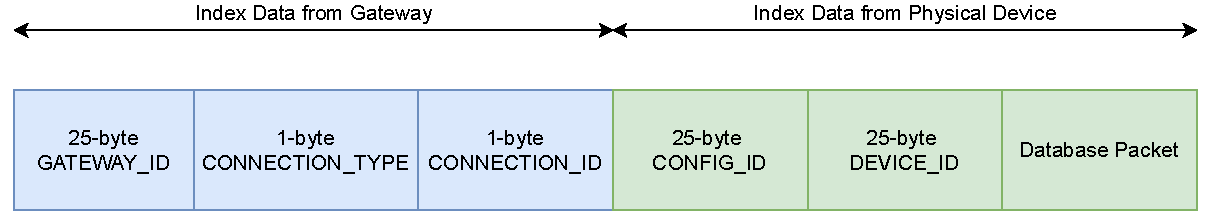
\includegraphics[width=1.0\linewidth]{images/Thesis-Page-12-Hardware-data-frame-struct.pdf}
\caption{Cấu trúc gói dữ liệu trên frame giao tiếp với phần cứng.}
\label{fig:Hardware-data-frame-struct}
\end{figure}

\subsubsection{Giao tiếp với giao diện web}

\acrshort{api} server đóng vai trò như một \acrfull{rest} \acrshort{api} và Websocket server trong giao tiếp với giao diện web.

Trong vai trò \acrshort{rest} \acrshort{api} server, ứng dụng server cung cấp các dịch vụ tương tác với database theo cấu trúc \acrfull{crud} và phong cách \acrshort{rest} (minh họa như bảng \ref{tab:CRUD-REST-service}). Dựa trên cấu trúc này, giao diện web có thể truy xuất database thông qua các phương thức \acrshort{http} với cấu trúc \acrshort{crud} tương ứng. Hiện tại, giao diện web có thể truy xuất tới 5 \acrshort{rest} \acrshort{api}. Đó là:

\begin{itemize}
    \item ``config'': dịch vụ truy xuất dữ liệu các cấu hình chung cho tất cả thiết bị phần cứng.
    \item ``device'': dịch vụ truy xuất dữ liệu của một thiết bị vật lý cụ thể.
    \item ``UI'': dịch vụ truy xuất dữ liệu của một UI dashboard linh hoạt.
    \item ``user'': dịch vụ truy xuất dữ liệu của một người dùng.
    \item ``vStorage'': dịch vụ truy xuất dữ liệu của một \acrshort{vs}.
\end{itemize}

\begin{table}[htp]
\caption{Cấu trúc CRUD theo phong cách REST. Nguồn từ Wikipedia~\cite{CRUD-REST-Service}.}

\label{tab:CRUD-REST-service}%
\begin{center}
\begin{tabular}{|l|l|}
\hline
\textbf{CRUD} & \textbf{HTTP} \\ \hline
Create        & POST, PUT     \\ \hline
Read          & GET           \\ \hline
Update        & PUT, PATCH    \\ \hline
Delete        & DELETE        \\ \hline
\end{tabular}
\end{center}
\end{table}

Trong vai trò Websocket server, \acrshort{api} server đồng bộ (đề cập ở mục \ref{VSync-Mecha}) các sự thay đổi dữ liệu database với giao diện web. Cụ thể, dựa trên sự kiện ``change streams'' của MongoDB, dữ liệu của các \acrshort{vs} sẽ luôn được thông báo tới giao diện web. Cấu trúc dữ liệu gửi tới giao diện web là kiểu dữ liệu \acrfull{json} (minh họa như hình \ref{fig:VSSync-JSON-model}). Trong đó:

\begin{itemize}
    \item Trường ``cmd'' là lệnh yêu cầu đồng bộ dự liệu \acrshort{vs}.
    \item Trường ``data'' là trường dữ liệu cần đồng bộ. Trường này chứa ID của \acrshort{vs} (\textbf{\_vs\_id}), device ID (\textbf{dev\_id}), dữ liệu đồng bộ (\textbf{data}), và toàn bộ thuộc tính của \acrshort{vs} (\textbf{fullDocument}).
\end{itemize}

\begin{figure}[htp]
\centering
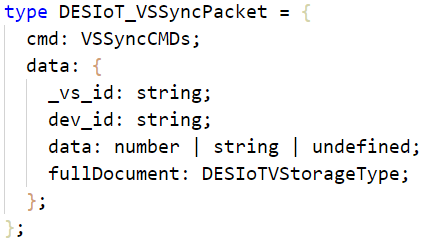
\includegraphics[width=0.5\linewidth,frame]{images/fig-Hardware-data-frame-struct.png}
\caption{Cấu trúc dữ liệu JSON đồng bộ với giao diện web.}
\label{fig:VSSync-JSON-model}
\end{figure}

\subsubsection{Giao tiếp với database}

\acrshort{api} server tạo kết nối với MongoDB thông qua thư viện MongooseJS. Cụ thể, ứng dụng server kết nối với MongoDB qua phương thức \textbf{mongoose.connect()}. Cuối cùng, mongoose cung cấp giải pháp đơn giản, dựa trên schema để lập mô hình (model) dữ liệu trên ứng dụng server \cite{Mongoose-Solution}. Các model trong giao tiếp này bao gồm:

\begin{itemize}
    \item ``config'': cấu trúc document của các cấu hình chung cho tất cả thiết bị phần cứng.
    \item ``device'': cấu trúc document của một thiết bị vật lý cụ thể.
    \item ``UI'': cấu trúc document của một UI dashboard linh hoạt.
    \item ``user'': cấu trúc document của một người dùng.
    \item ``vStorage'': cấu trúc document của một \acrshort{vs}.
\end{itemize}

\subsection{MongoDB}

MongoDB là một hệ quản trị cơ sở dữ liệu miễn phí và mã nguồn mở đa nền tảng. Được phân loại như một hệ quản trị cơ sở dữ liệu NoSQL, MongoDB sử dụng các \acrshort{json}-like document với schema~\cite{MongoDB-Def}. Trên \acrshort{vps}, MongoDB hoạt động như một ứng dụng server. Cụ thể, ứng này được cài đặt bằng ``mongo Docker Image'' trên \textbf{docker-compose} và hoạt động trên cùng một \acrshort{vlan} với \acrshort{api} server và \acrshort{mqtt} Broker.

% connect and change streams
MongoDB thiết lập kết nối với \acrshort{api} server thông qua thư viện ``MongooseJS'' và cung cấp giải pháp cho việc đồng bộ với phần cứng và giao diện web. Cụ thể, MongoDB cung cấp giải pháp đồng bộ thông qua sự kiện ``change streams''. Sự kiện này giúp ứng dụng server theo dõi các thay đổi dữ liệu thời gian thực một cách dễ dàng. ``Change streams'' hoạt động trên ``Replica set'' của MongoDB.

% Replica set
Trên \acrshort{vps}, Mongo được triển khai trên mô hình ``Replica set''. Một \textit{replica set} trong MongoDB là một tập hợp các \textit{mongod} process mà duy trì cùng một data set. \textit{Replica set} cung cấp tính dự phòng (redundancy) và có sẵn cao (high availability), và là cơ sở cho tất cả quá trình phát triển sản phẩm~\cite{Mongo-Replication-Def}. Trên \acrshort{vps}, mô hình MongoDB \textit{Replica set} (minh họa như hình \ref{fig:MongoDB-Replication-Model}) bao gồm một \textit{primary} node và hai \textit{secondary} node.

\begin{figure}[htp]
\centering
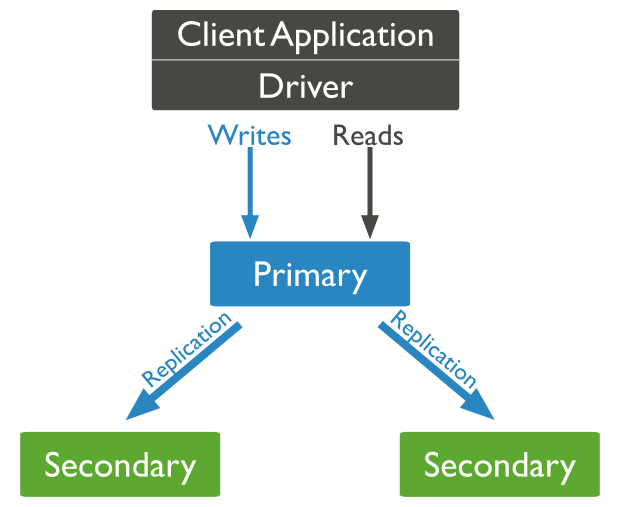
\includegraphics[width=0.7\linewidth]{images/replica-set-read-write-operations-primary.bakedsvg.png}
\caption{Mô hình MongoDB Replica Set trên VPS. Nguồn từ MongoDB~\cite{Mongo-Replication-Def}.}
\label{fig:MongoDB-Replication-Model}
\end{figure}

\section{Giao diện web}

%  Tổng quan
Giao diện web được xây dựng trên nền tảng Ant Design Pro, framework ReactJS, và ngôn ngữ TypeScript. Dựa trên nền tảng này, giao diện web sẽ được phát triển để cung cấp tương tác cho các admin dựa trên thư viện Ant Design và framework UmiJS.
% Những thành phần chính trên giao diện
Trên nền tảng Ant Design Pro, giao diện được trang bị sẵn Main Page (minh họa như hình \ref{fig:adp-default-mainpage}) và Login Page \ref{fig:adp-default-loginpage}). Main Page Layout bao gồm Page Header, Menu, Menu Header, Right Content, và Page Content; và Login Page cung cấp form để đăng nhập.

\begin{figure}[htp]
\centering
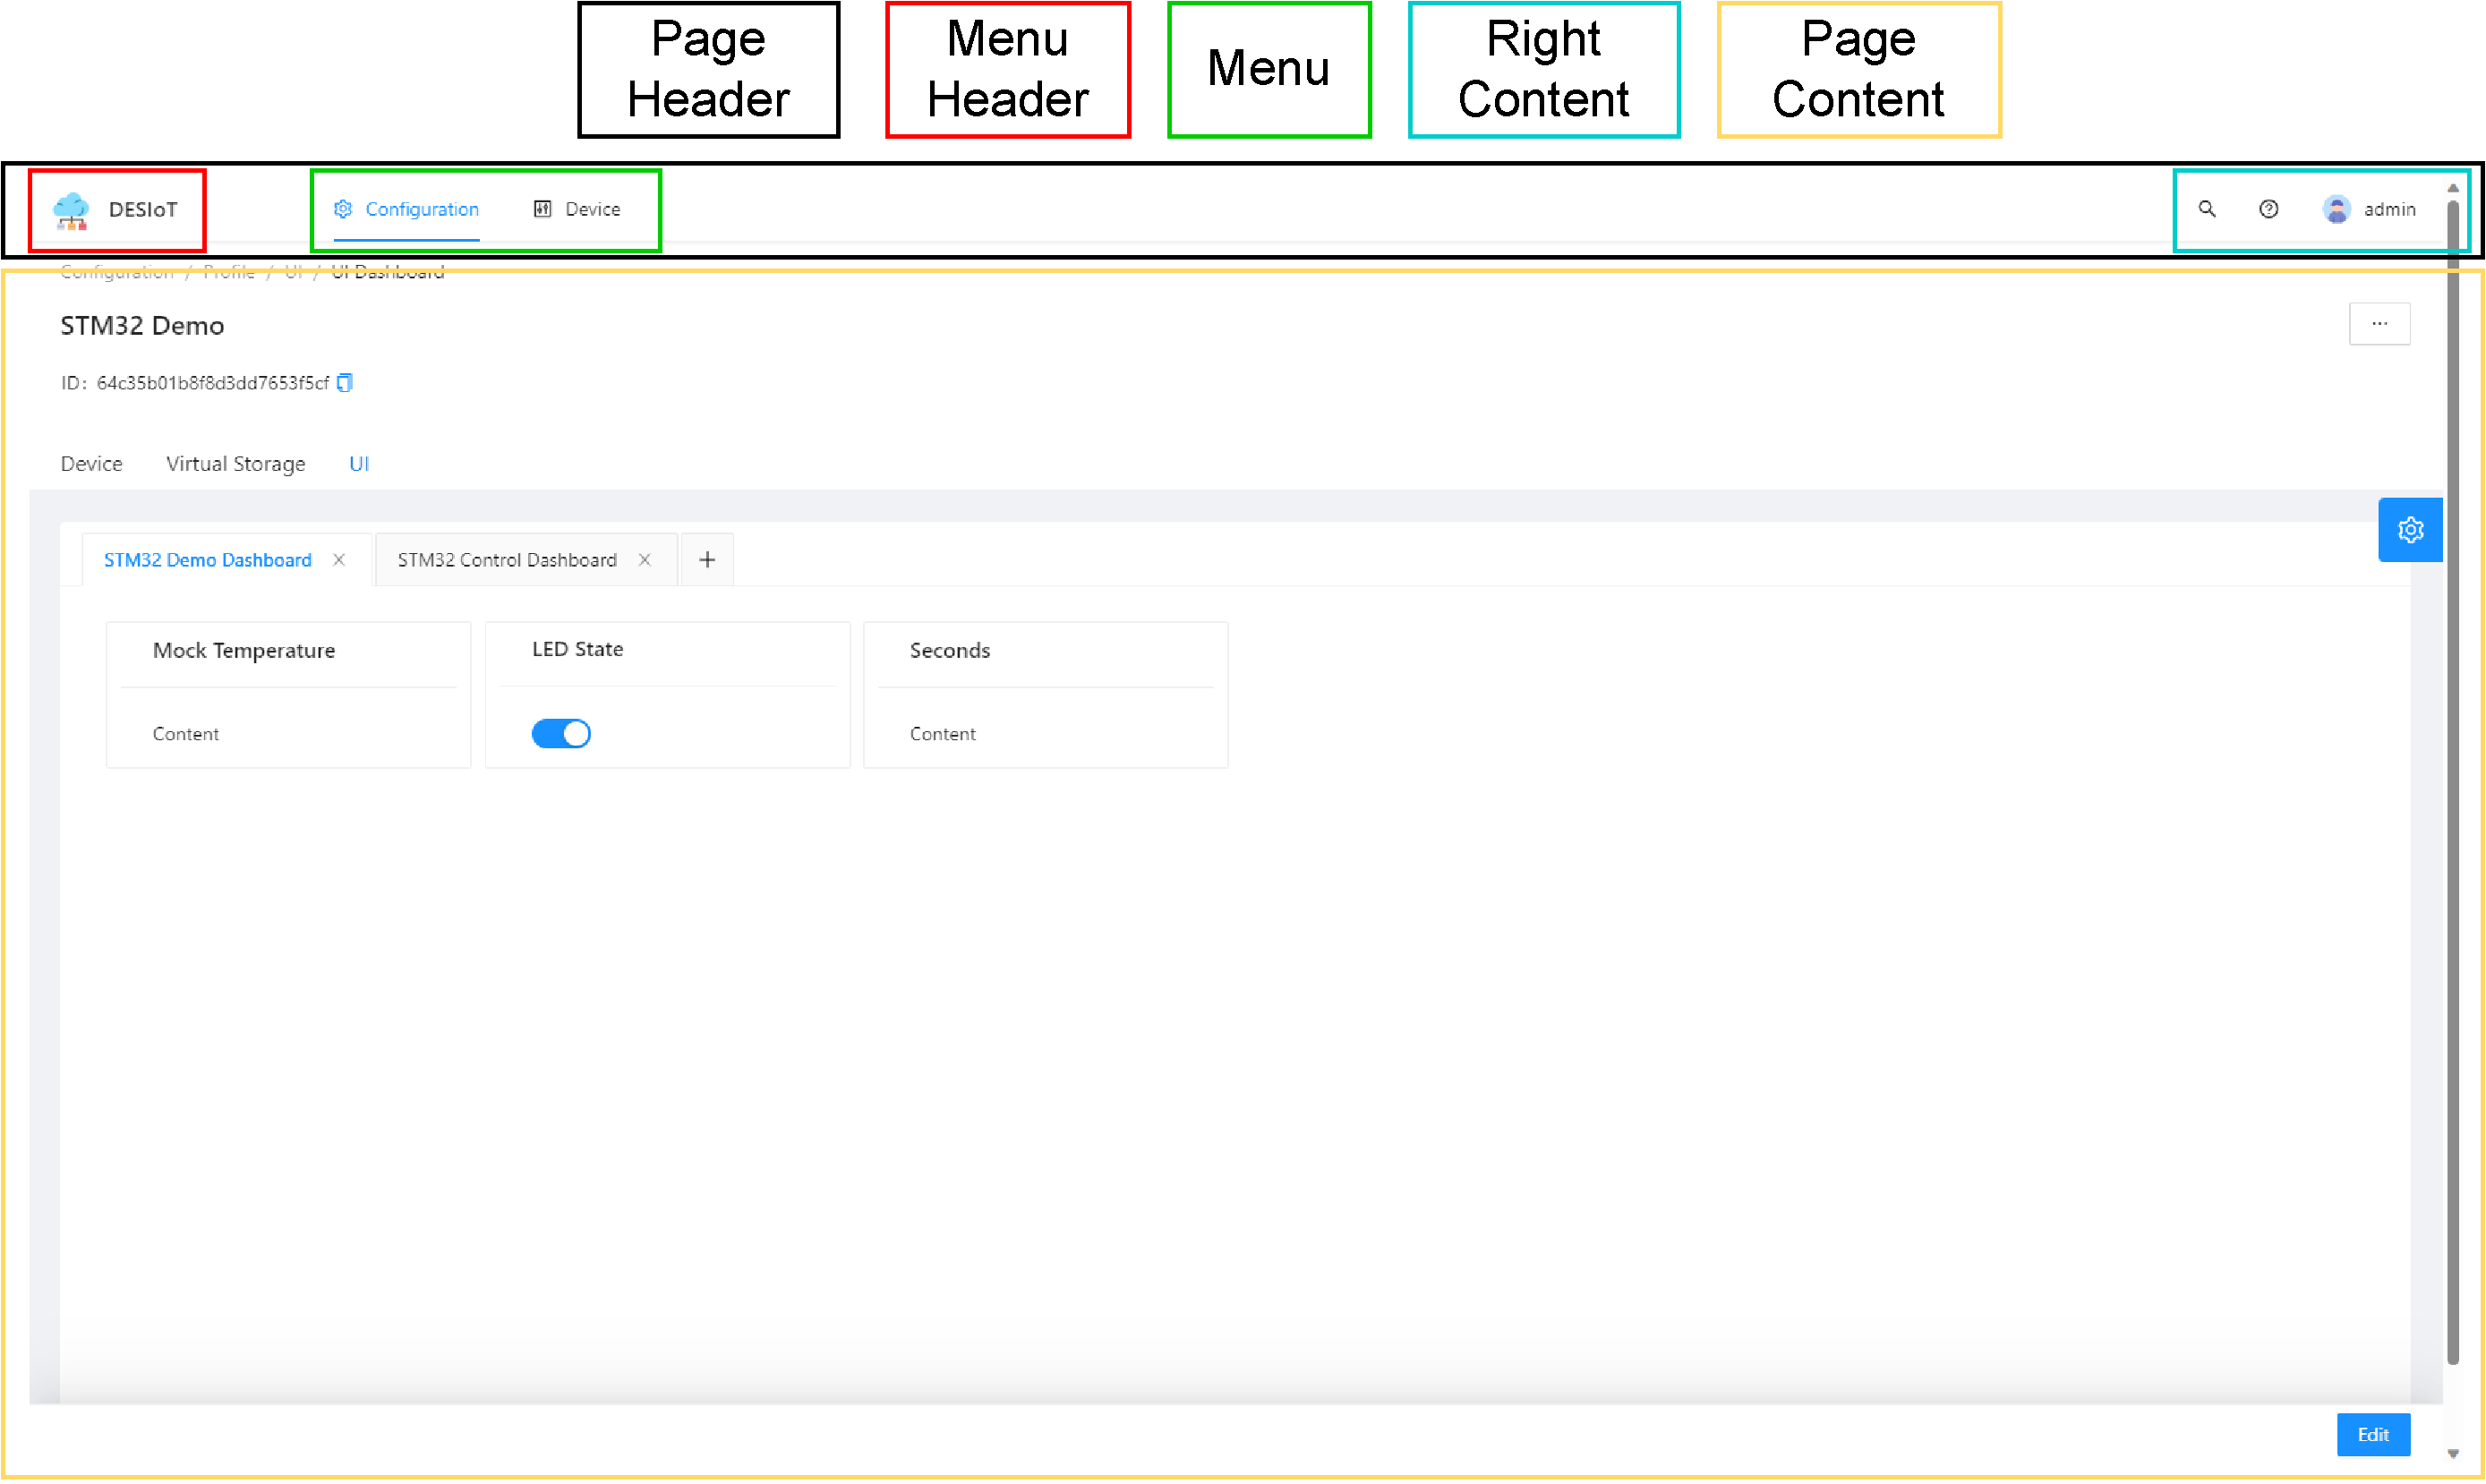
\includegraphics[width=1.0\linewidth]{images/Thesis-Page-13-adp-default-mainpage.pdf}
\caption{Layout của Main Page trên nền tảng Ant Design Pro.}
\label{fig:adp-default-mainpage}
\end{figure}

\begin{figure}[htp]
\centering
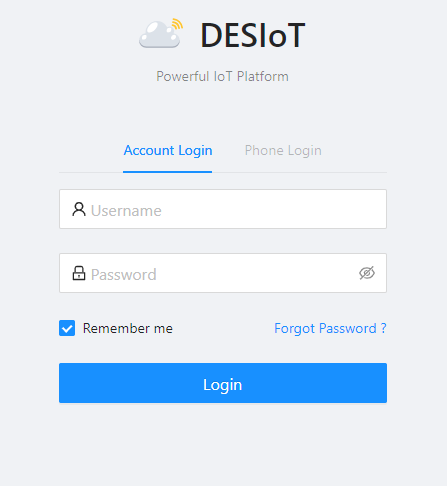
\includegraphics[width=0.7\linewidth]{images/fig-adp-default-loginpage.png}
\caption{Login Page trên nền tảng Ant Design Pro.}
\label{fig:adp-default-loginpage}
\end{figure}

% Các tương tác thiết lập trên giao diện web
Dựa trên nền tảng Ant Design Pro, giao diện web thiết lập các tương tác cho các quản trị viên. Các tương tác này chủ yếu diễn ra trên hai trang Configuration và Device.

\subsection{Configuration Page}

Configuration Page (minh họa như hình \ref{fig:config-page}) hiển thị và cung cấp tương tác cho các cấu hình trên thiết bị phần cứng. Cụ thể, trên trang này, người dùng có thể quan sát, tạo mới, và truy cập một configuration.

\begin{figure}[htp]
\centering
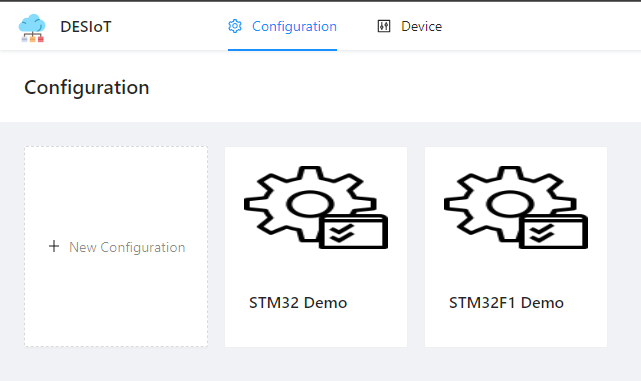
\includegraphics[width=0.7\linewidth]{images/fig-config-page.png}
\caption{Giao diện của Configuration Page.}
\label{fig:config-page}
\end{figure}

% Các tab
Khi mở một trang của một Configuration, người dùng có thể xem thông tin của Configuration. Ngoài ra, Configuration Page còn cung cấp các tab Device, Virtual Storage, và UI. Các tab này giúp truy xuất cơ sở dữ liệu trên model của một thiết bị phần cứng, \acrshort{vs}, và UI dashboard.

Trên tab Device, Device Tab (minh họa như hình \ref{fig:config-device-tab}) hiển thị danh sách thiết bị và người dùng có thể tạo mới hoặc xóa dữ liệu của một thiết bị thông qua \textbf{Add device} hoặc \textbf{Delete} button tương ứng. Dữ liệu của một device bao gồm ``Name'' và ``ID''.

\begin{figure}[htp]
\centering
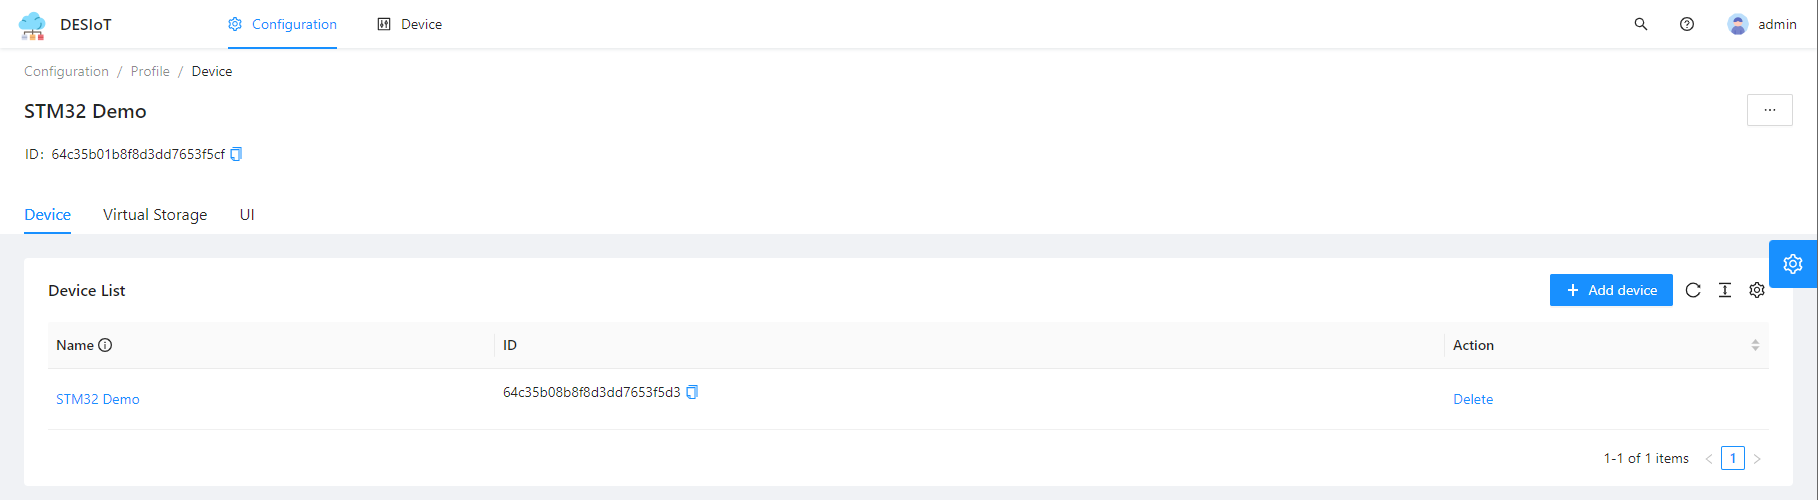
\includegraphics[width=1.0\linewidth]{images/fig-config-device-tab.png}
\caption{Giao diện của Device Tab trên Configuration Page.}
\label{fig:config-device-tab}
\end{figure}

Trên tab Virtual Storage, Virtual Storage Tab (minh họa như hình \ref{fig:config-vstorage-tab}) hiển thị danh sách các \acrshort{vs} và người dùng có thể tạo mới hoặc xóa dữ liệu của một \acrshort{vs} thông qua \textbf{Add Virtual Storage} hoặc \textbf{Delete} button tương ứng. Dữ liệu của một \acrshort{vs} bao gồm ``Name'', ``VStorage ID'', và ``Data Type''.

\begin{figure}[htp]
\centering
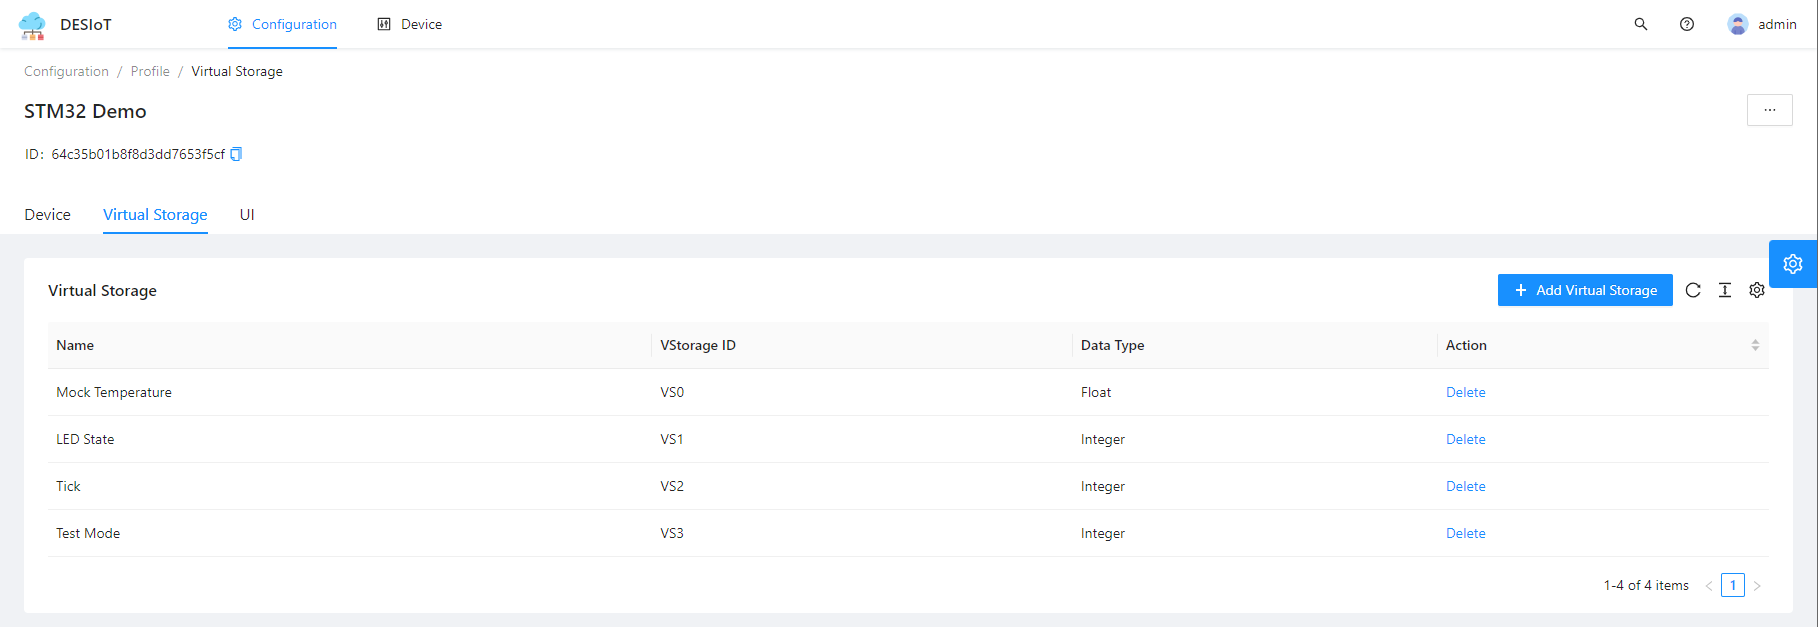
\includegraphics[width=1.0\linewidth]{images/fig-config-vstorage-tab.png}
\caption{Giao diện của Virtual Storage Tab trên Configuration Page.}
\label{fig:config-vstorage-tab}
\end{figure}

Trên tab UI, UI Tab (minh họa như hình \ref{fig:config-ui-tab}) hiển thị danh sách các Dashboard tab và người dùng có thể tạo mới hoặc xóa dữ liệu của một Dashboard thông qua ``+'' hoặc ``X'' button tương ứng. Trên mỗi Dashboard, người dùng có thể bật chế độ chỉnh sửa (minh họa như hình \ref{fig:config-ui-tab-edit-mode}) thông qua \textbf{Edit} button. Trên chế độ này, người dùng có thể thêm, xóa, hoặc chỉnh sửa các widget có sẵn để thiết kế Dashboard.

\begin{figure}[htp]
\centering
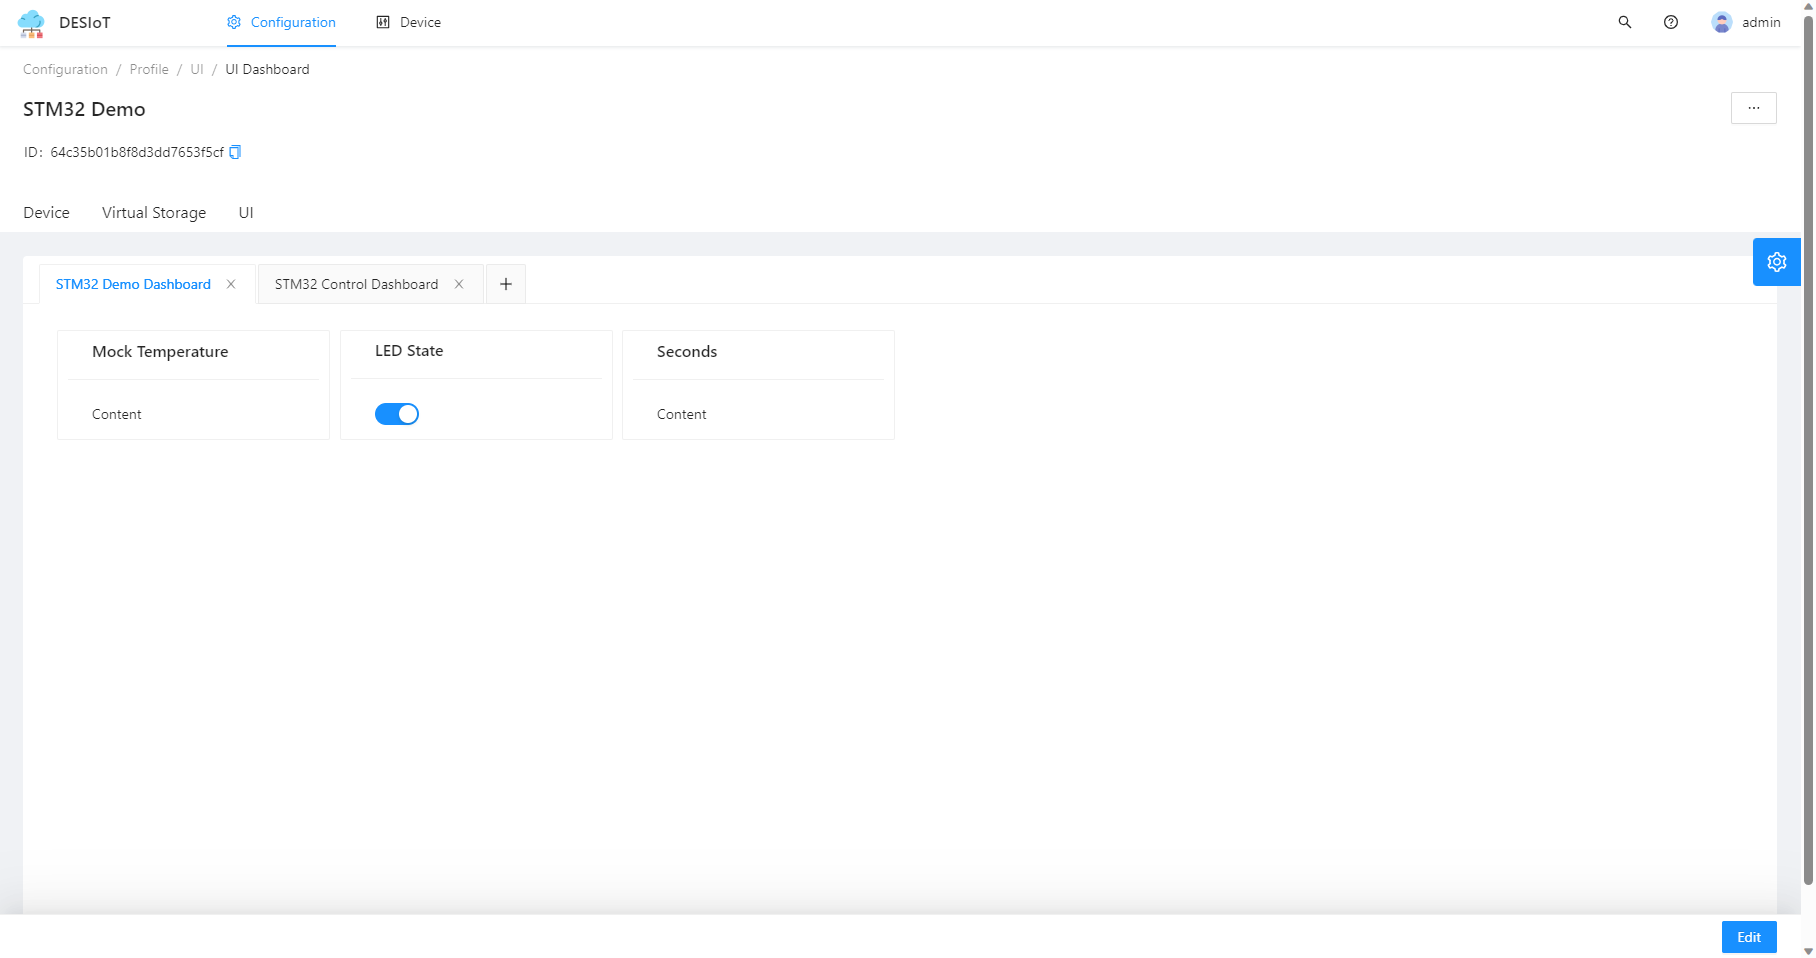
\includegraphics[width=1.0\linewidth]{images/fig-config-ui-tab.png}
\caption{Giao diện của UI Tab trên Configuration Page.}
\label{fig:config-ui-tab}
\end{figure}

\begin{figure}[htp]
\centering
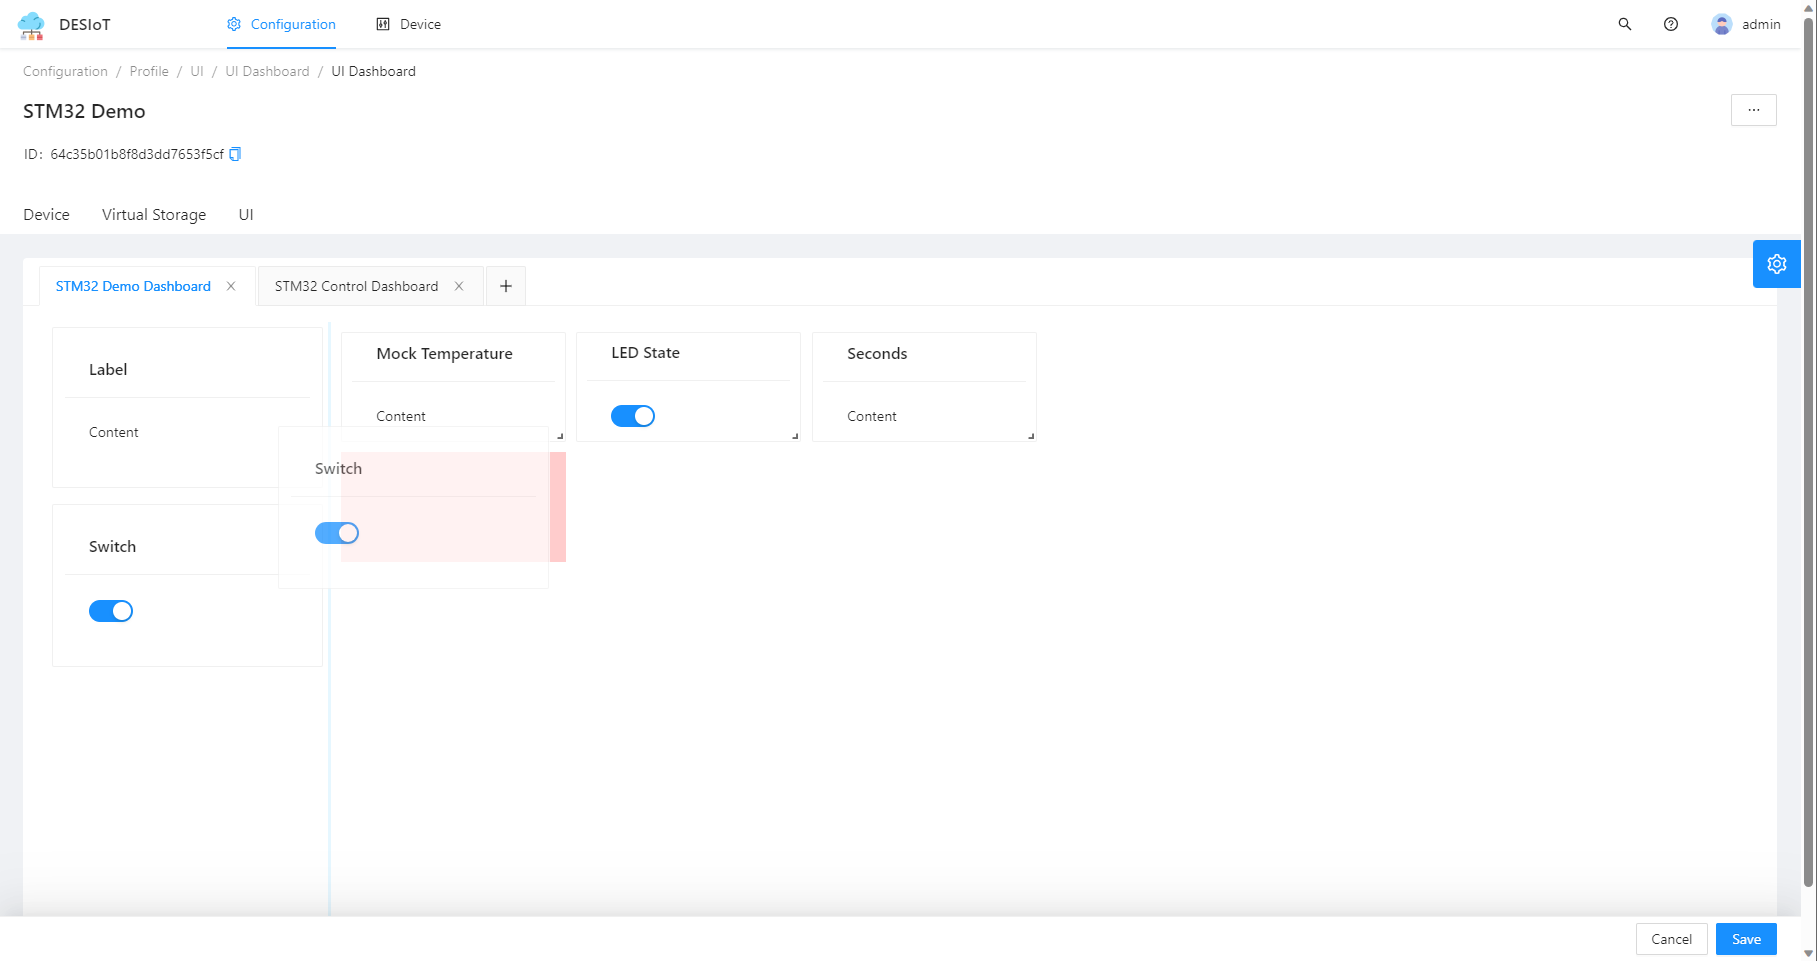
\includegraphics[width=1.0\linewidth]{images/fig-config-ui-tab-edit-mode.png}
\caption{Giao diện của UI Tab chế độ Edit trên Configuration Page.}
\label{fig:config-ui-tab-edit-mode}
\end{figure}

\subsection{Device Page}

Device Page (minh họa như hình \ref{fig:device-page}) hiển thị danh sách các thiết bị đã cấu hình trên Configuration Page. Khi mở một Device Tab, người dùng có thể lựa chọn UI Dashboard đã tạo và quan sát dữ liệu thời gian thực và điều khiển thiết bị trên dashboard.

\begin{figure}[htp]
\centering
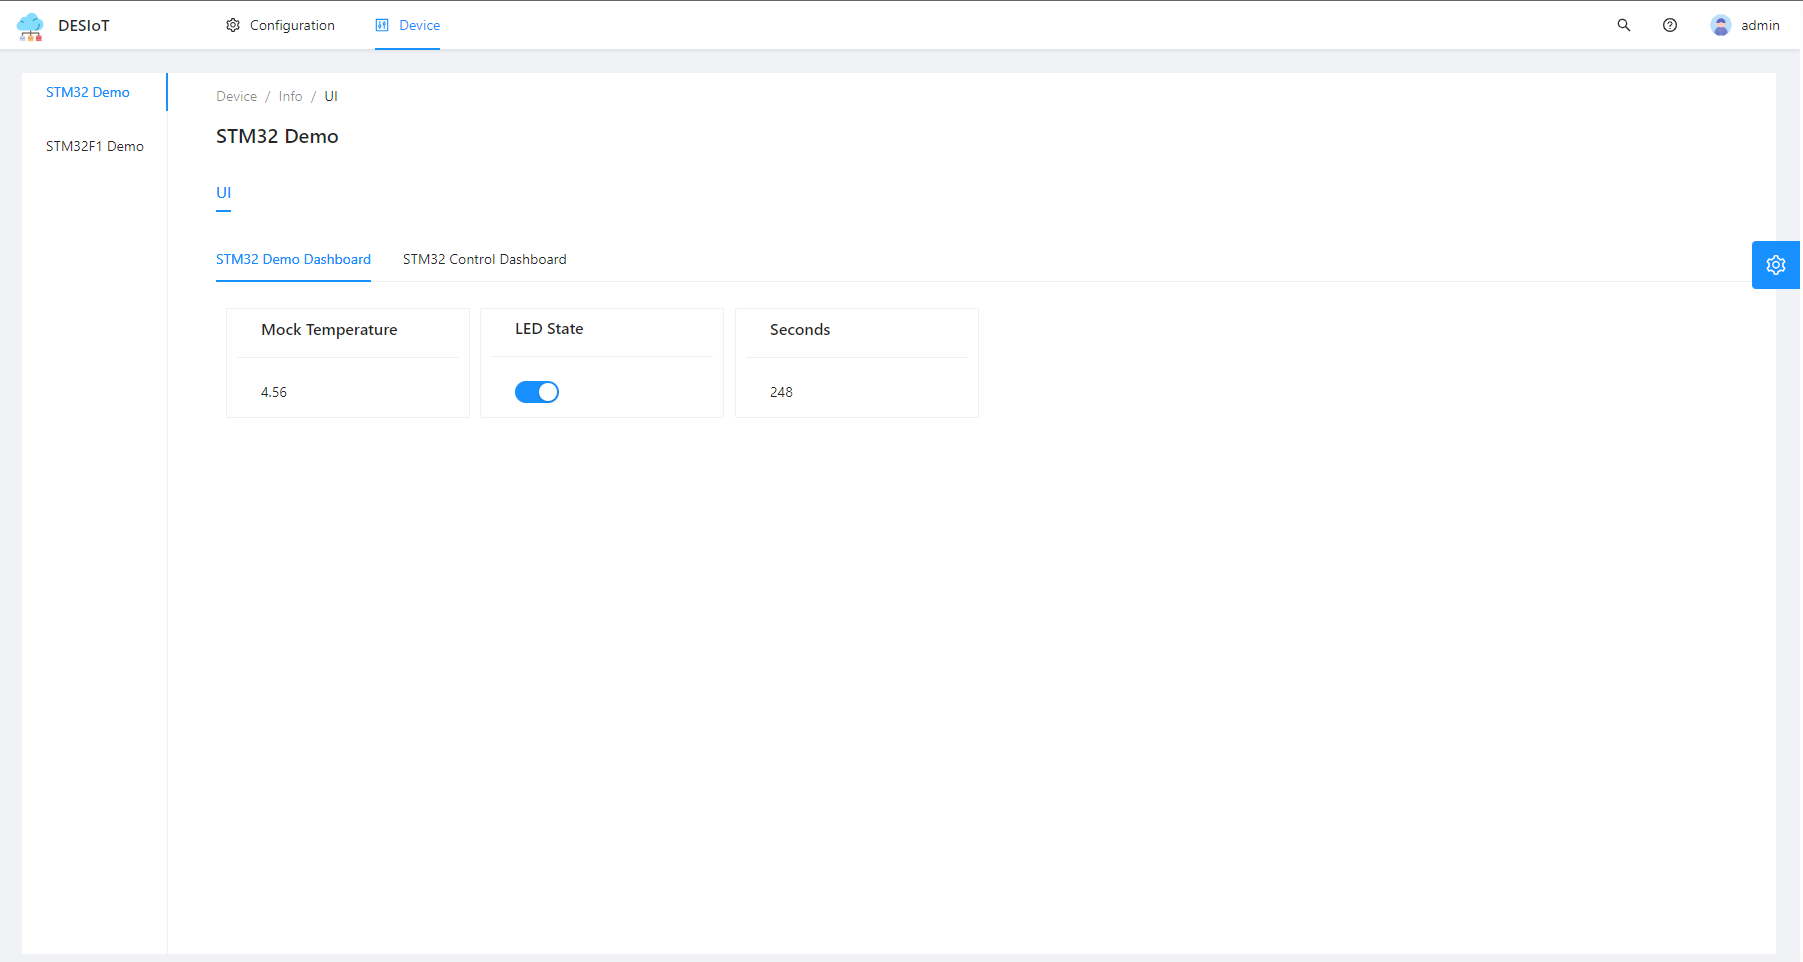
\includegraphics[width=1.0\textheight,angle=90,frame]{images/fig-device-page.png}
\caption{Giao diện của Device Page.}
\label{fig:device-page}
\end{figure}

\chapter{KẾT QUẢ}
\label{Chapter4}


\chapter{Kết luận}
\label{Chapter5}

% Công trình của tác giả (nếu không có thì comment 02 dòng dưới)
\phantomsection
\addcontentsline{toc}{chapter}{DANH MỤC CÔNG TRÌNH CỦA TÁC GIẢ}
\chapter*{DANH MỤC CÔNG TRÌNH CỦA TÁC GIẢ}
\label{Appendix1}

\begin{enumerate}
\item Nguyễn Tiến Đạt,Nguyễn Vũ Minh Thành,Đỗ Đức Phú,Nguyễn Văn Nhị,Lê Đức Hùng, (2022), ``Thực hiện thuật toán ChaCha20 - Poly1305
trên phần cứng ứng dụng bảo mật hệ thống IoT'', \textit{Hội nghị Quốc gia về Điện tử, Truyền thông và Công nghệ Thông tin lần thứ XXV, REV-ECIT 2022}.
\end{enumerate}

% In tài liệu tham khảo
\phantomsection
\addcontentsline{toc}{chapter}{TÀI LIỆU THAM KHẢO}
\printbibheading[title={TÀI LIỆU THAM KHẢO}]

% \printbibliography[heading=subbibliography, title={Tiếng Việt}, keyword=Viet, resetnumbers=true]

\DeclareNameAlias{sortname}{last-first}
\DeclareNameAlias{default}{last-first}

\printbibliography[heading=subbibliography, title={Tiếng Anh}, notkeyword=Viet, resetnumbers=1] 
% ===================================================================== %
% CHÚ Ý: phải gán lại resetnumbers=số tài liệu tham khảo tiếng Việt + 1 %
% ===================================================================== %

% Phần phụ lục
% \appendix

\chapter{Ngữ pháp tiếng Việt}
\label{Appendix1}

Đây là phụ lục.
% \chapter{Ngữ pháp tiếng Nôm}
\label{Appendix2}

Đây là phụ lục 2.

\end{document} 